% !TeX root = ../main.tex
\documentclass[./../main.tex]{subfiles}

\begin{document}

\subsection{Môi trường phát triển}

\begin{itemize}
	\item Công cụ thiết kế giao diện người dùng: Figma, tổng cộng khoảng 30 màn hình chính
	\item Hệ điều hành: Ubuntu 20.04.3 LTS
	\item Ngôn ngữ lập trình: TypeScript
	\item Công cụ lập trình: Visual Studio Code
	\item Nền tảng sử dụng: React, thư viện Material UI
\end{itemize}

\subsection{Môi trường thực nghiệm}

\begin{itemize}
	\item Dịch vụ web hosting Gitlab Pages
\end{itemize}

\subsection{Kết quả thực nghiệm}

Phần này mô tả lại một vài luồng hoạt động chính của sinh viên, giảng viên, đối tác, quản trị viên Khoa và quản trị viên hệ thống.

\subsubsection{Luồng sử dụng của sinh viên}

\paragraph*{Sinh viên đọc bài đăng}

\begin{itemize}
	\item Hình \ref{fig:student_home_page}: Sinh viên truy cập trang chủ và chọn bài đăng muốn đọc.
	\item Hình \ref{fig:student_read_post_page}: Giao diện hiển thị bài đăng đã chọn.
\end{itemize}

\begin{figure}[]
	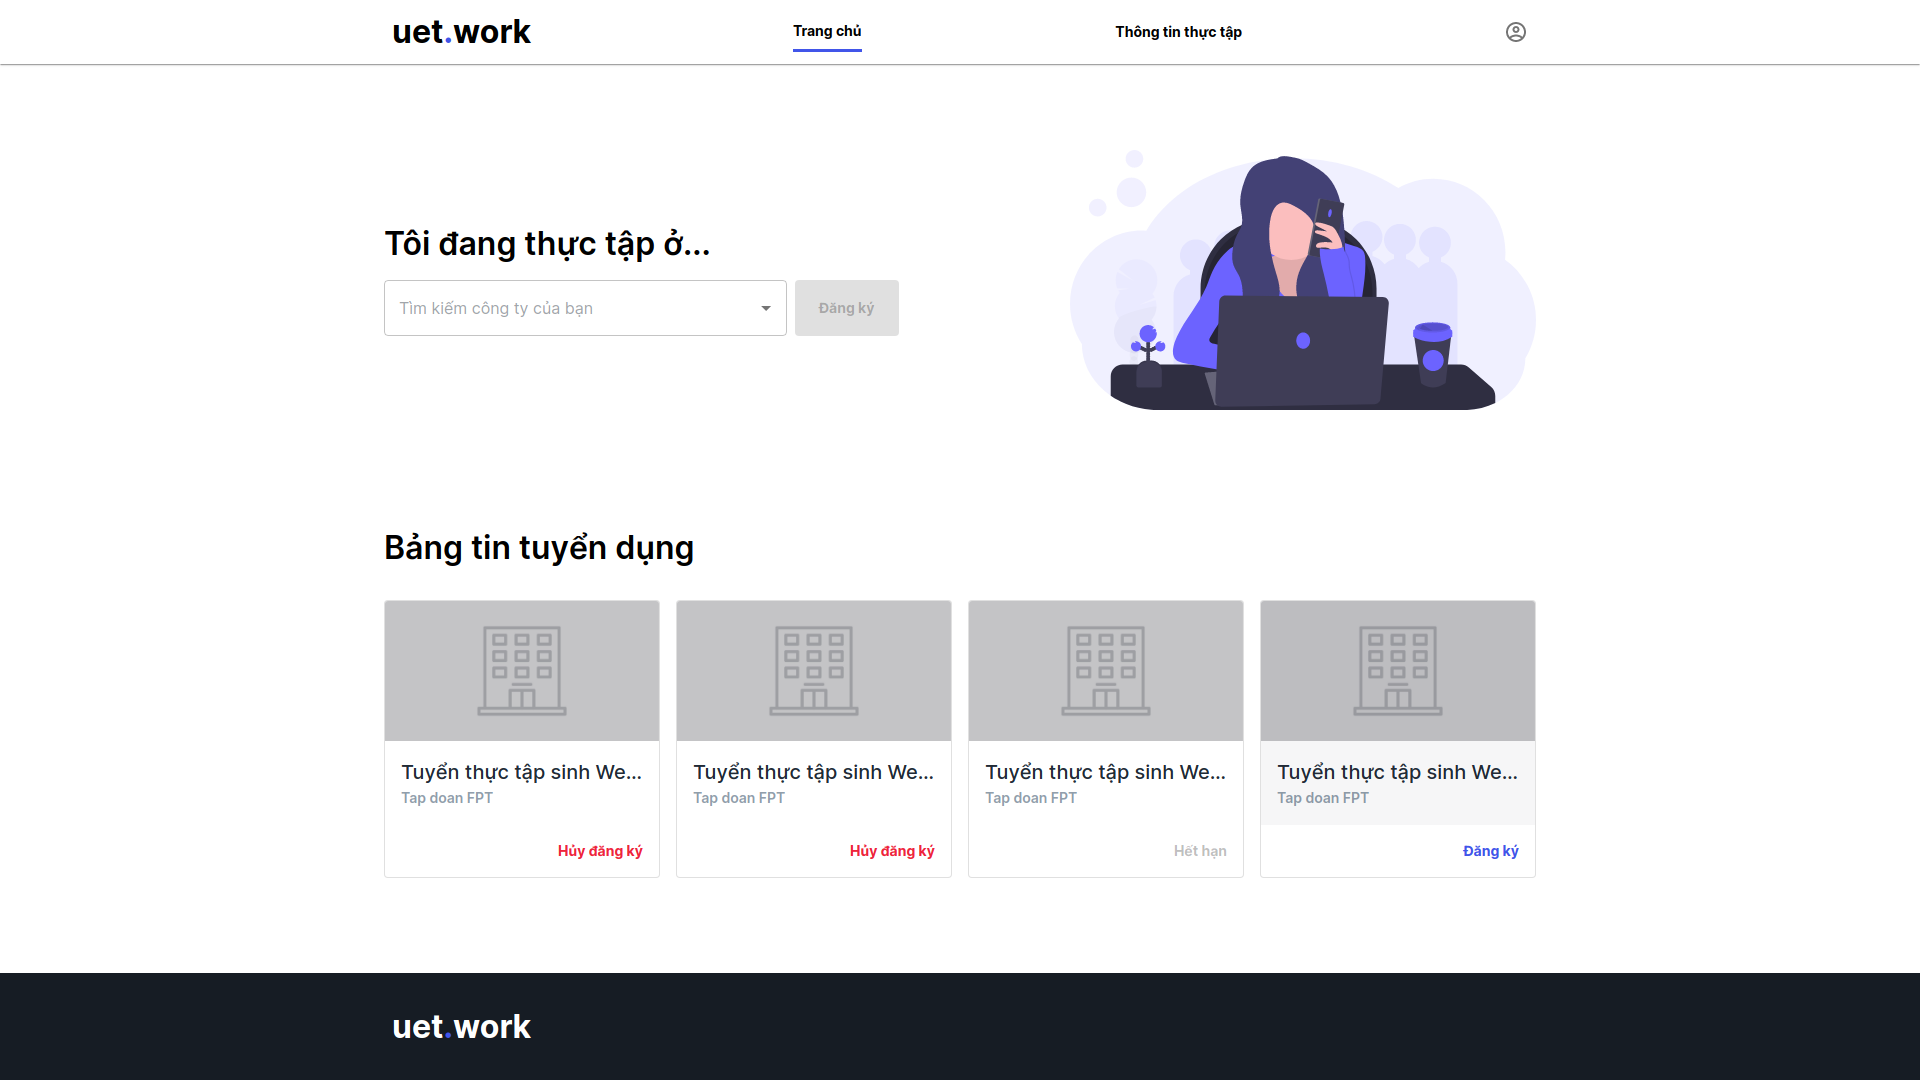
\includegraphics[width=\linewidth]{./images/image37.png}
	\caption{Luồng \emph{Đọc bài đăng}: Truy cập trang chủ và chọn bài đăng muốn đọc}
	\label{fig:student_home_page}
\end{figure}

\begin{figure}[]
	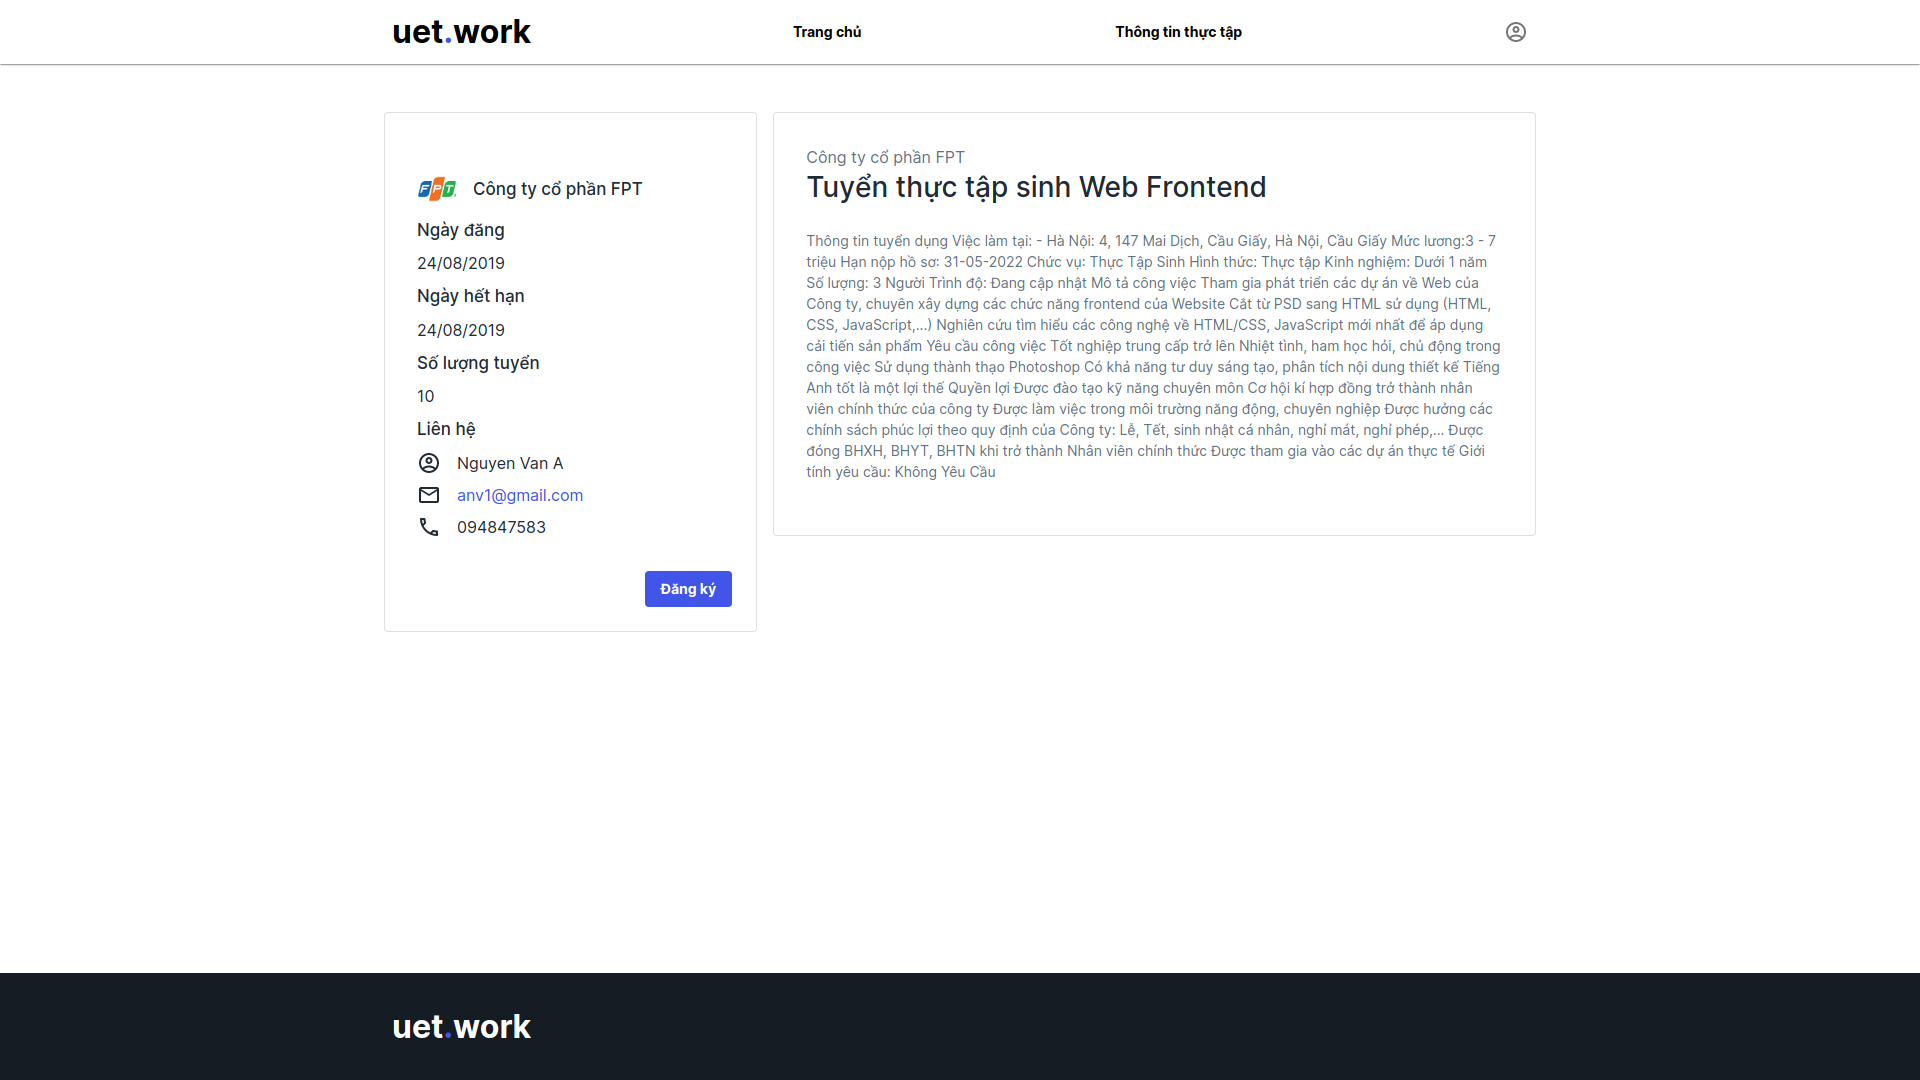
\includegraphics[width=\linewidth]{./images/image81.png}
	\caption{Luồng \emph{Đọc bài đăng}: Giao diện hiển thị bài đăng đã chọn}
	\label{fig:student_read_post_page}
\end{figure}

\paragraph*{Sinh viên đăng ký thực tập}

\begin{itemize}
	\item Hình \ref{fig:student_find_company}: Sinh viên tìm kiếm công ty mà mình đang thực tập và đăng ký.
	\item Hình \ref{fig:student_register_company_success}: Nếu thành công, hệ thống hiển thị thông báo đăng ký thành công.
	\item Hình \ref{fig:student_register_company_failed}: Nếu thất bại, hệ thống hiển thị thông báo đăng ký thất bại.
\end{itemize}

\begin{figure}[]
	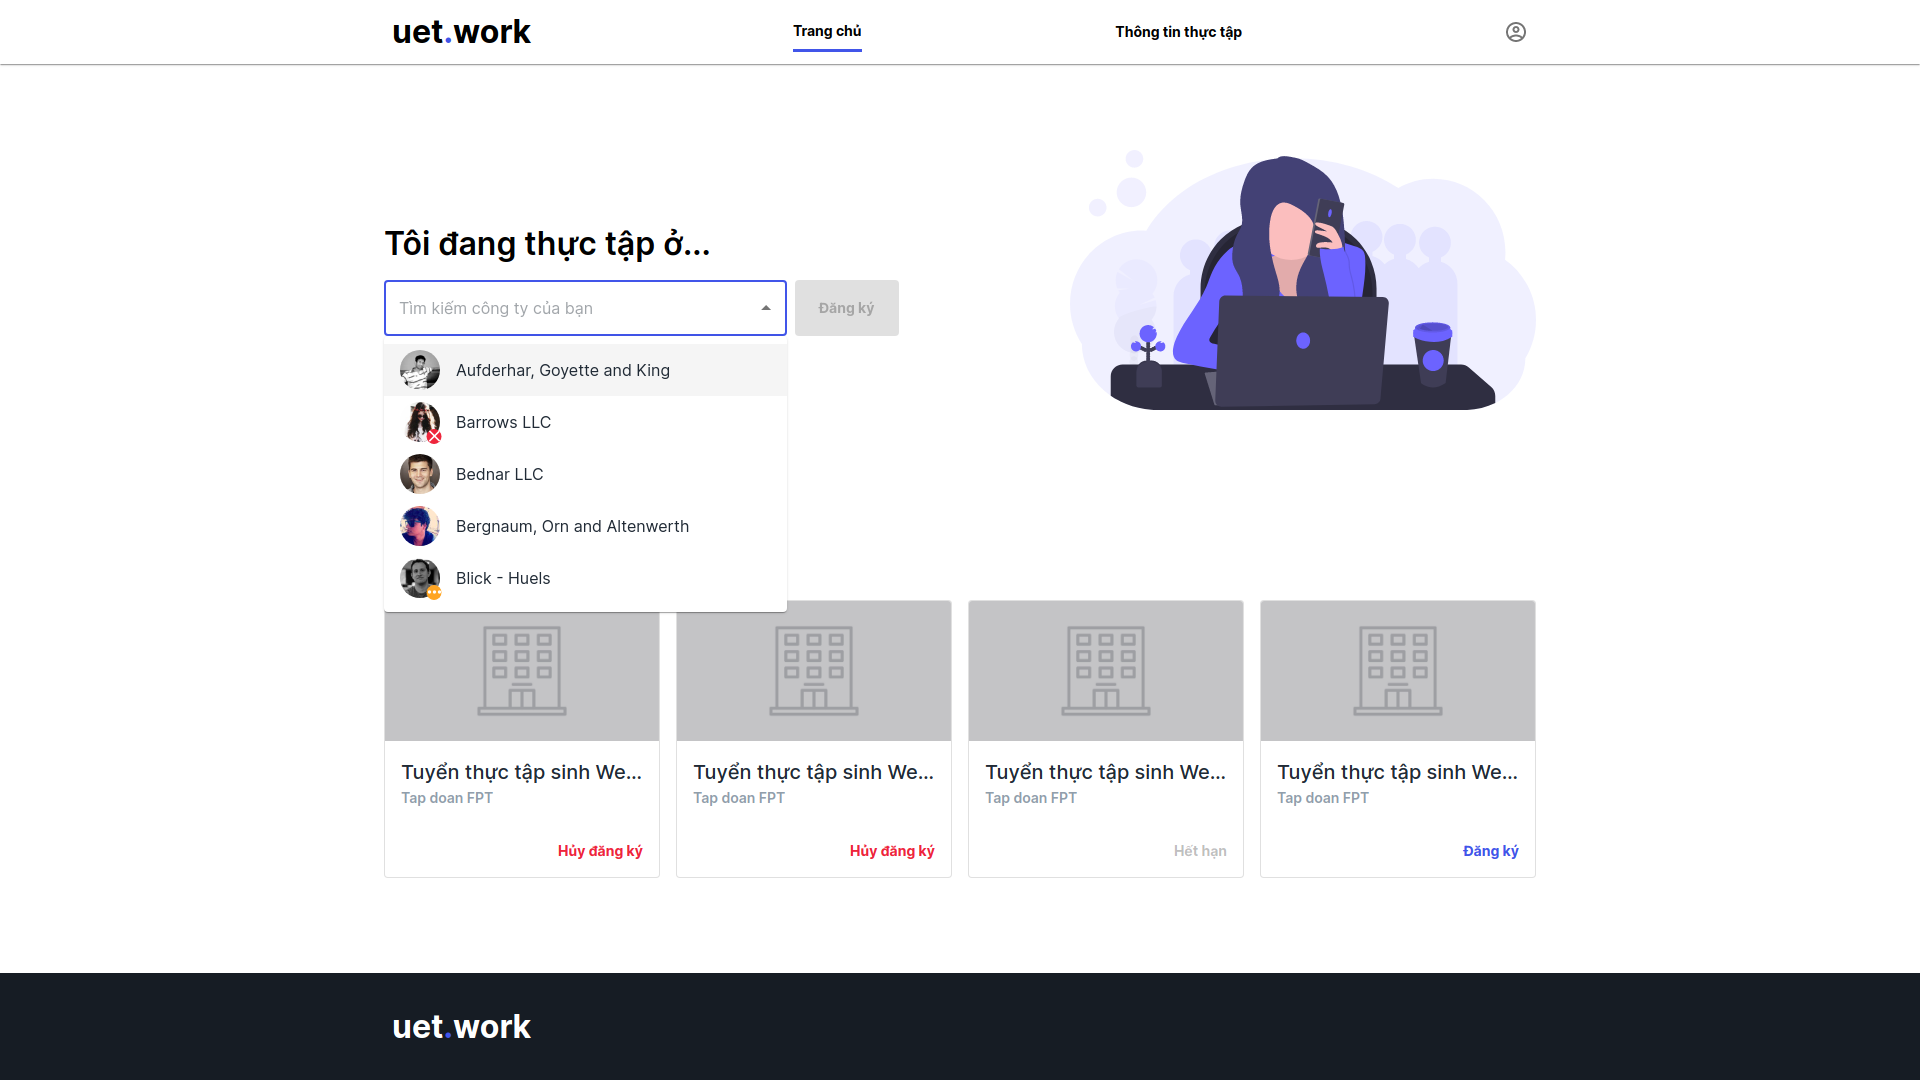
\includegraphics[width=\linewidth]{./images/image39.png}
	\caption{Luồng \emph{Sinh viên đăng ký thực tập}: Tìm kiếm công ty}
	\label{fig:student_find_company}
\end{figure}

\begin{figure}[]
	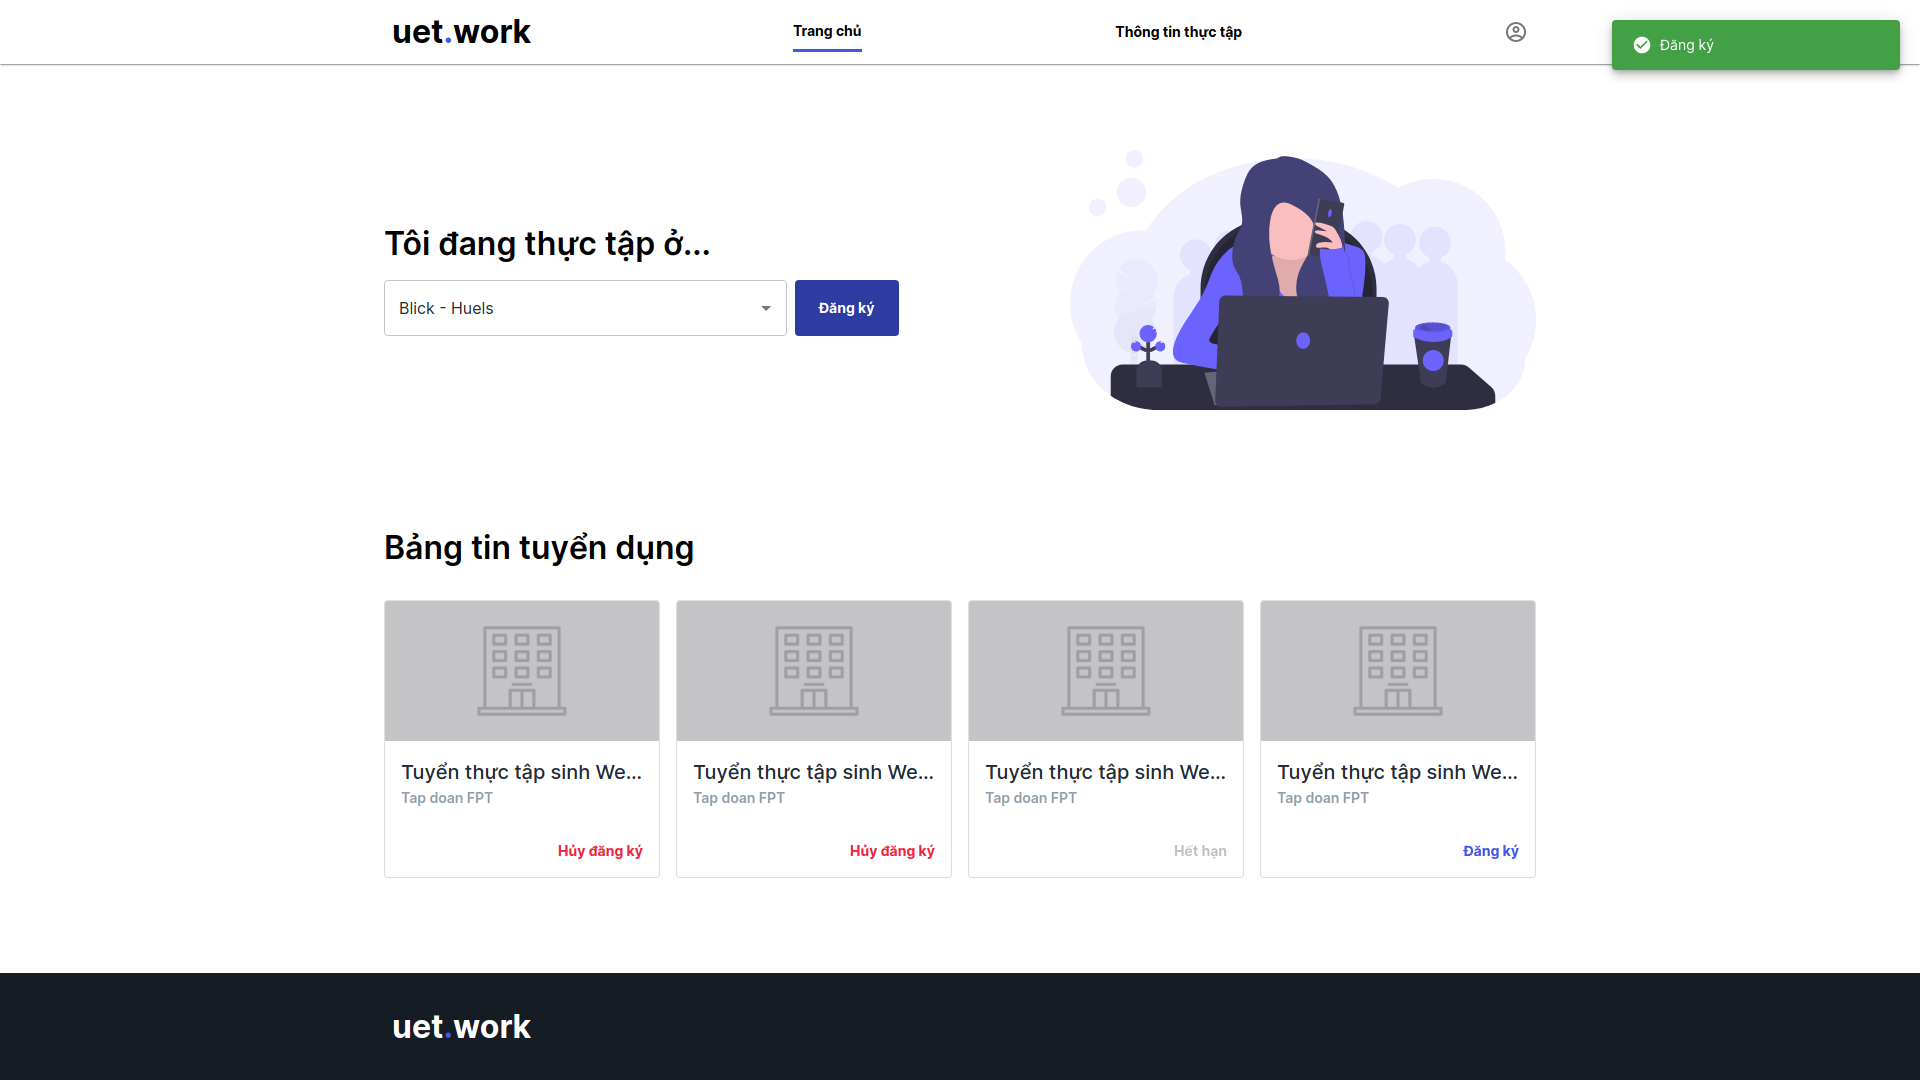
\includegraphics[width=\linewidth]{./images/image40-1.png}
	\caption{Luồng \emph{Sinh viên đăng ký thực tập}: Đăng ký thành công}
	\label{fig:student_register_company_success}
\end{figure}

\begin{figure}[]
	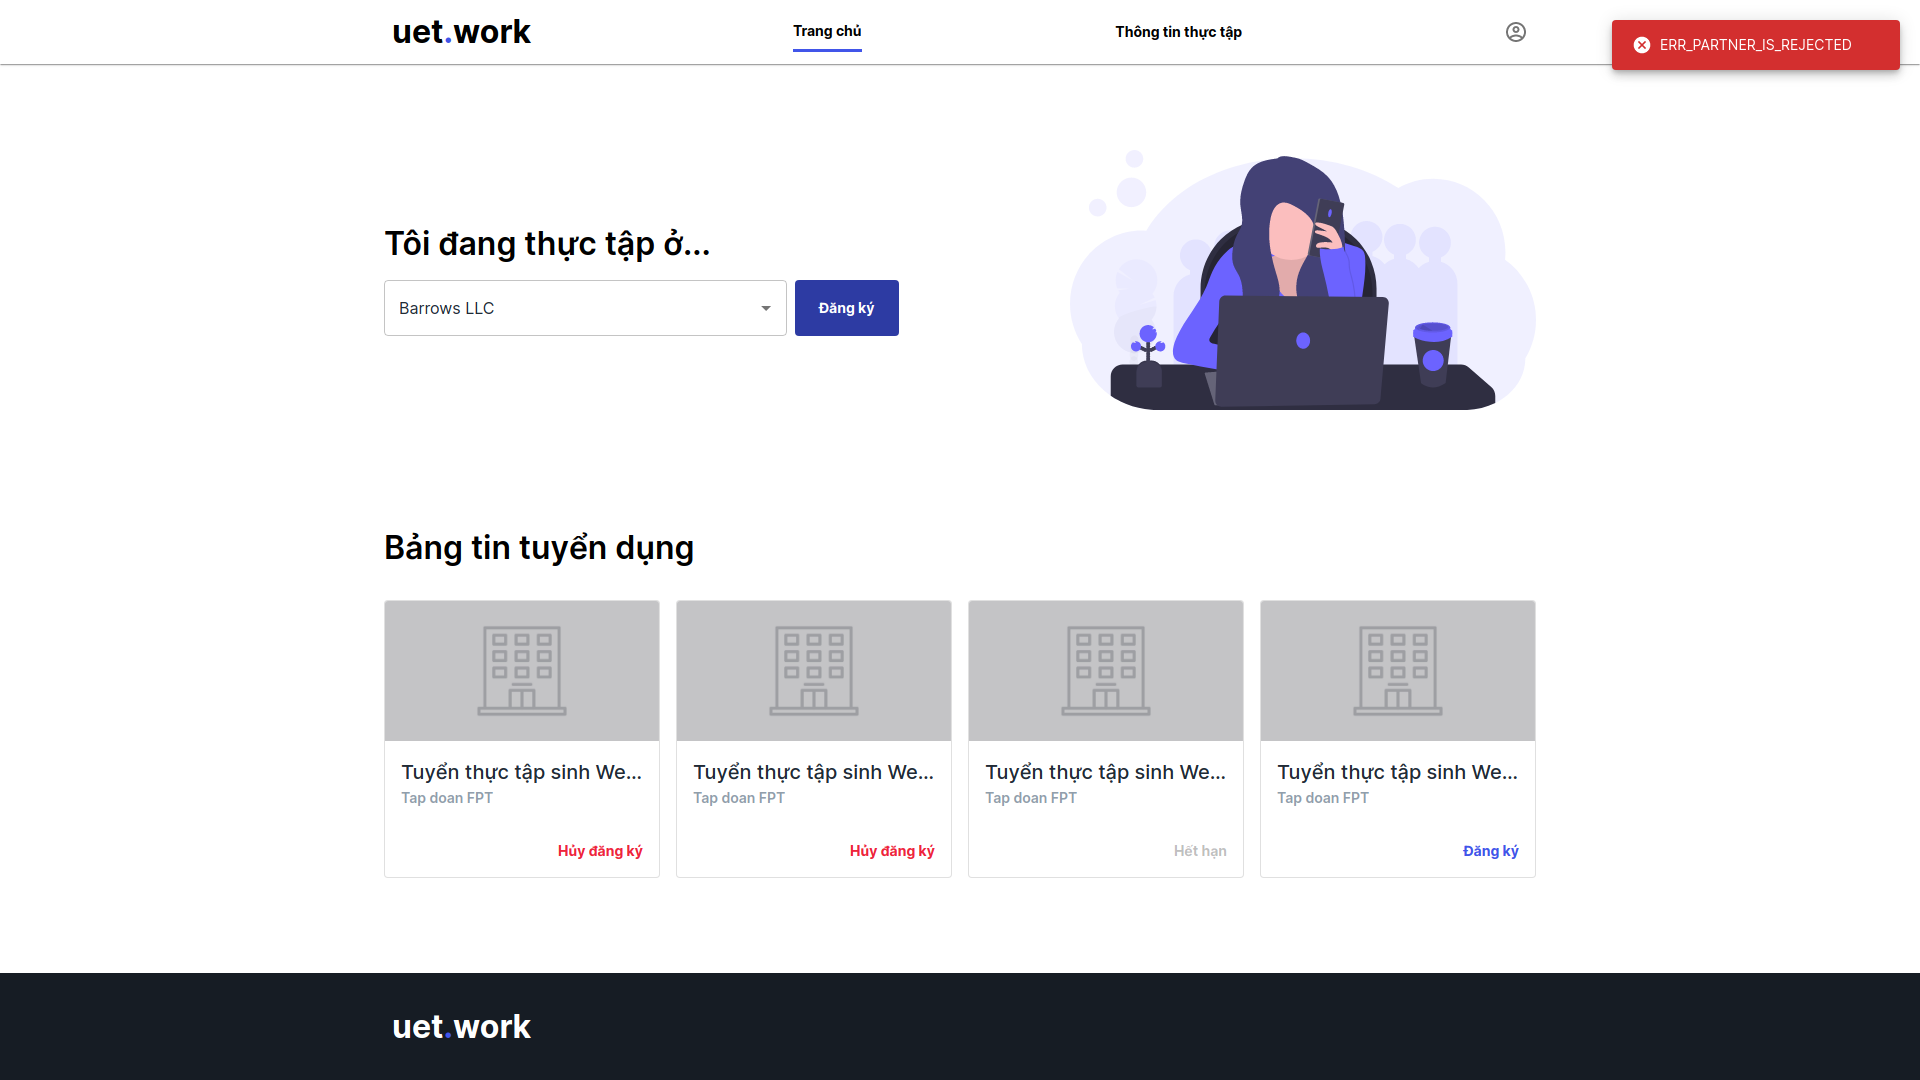
\includegraphics[width=\linewidth]{./images/image40.png}
	\caption{Luồng \emph{Sinh viên đăng ký thực tập}: Đăng ký thất bại}
	\label{fig:student_register_company_failed}
\end{figure}

\paragraph*{Sinh viên xem thông tin thực tập}
Sau khi đăng ký thực tập thành công, sinh viên vào kiểm tra thông tin thực tập của bản thân. Tại đây, sinh viên có thể xem thông tin công ty thực tập đã đúng chưa, giảng viên hướng dẫn là ai, và nộp báo cáo.

Hình \ref{fig:view_internship_page} mô tả màn hình trang thông tin thực tập.

\begin{figure}[]
	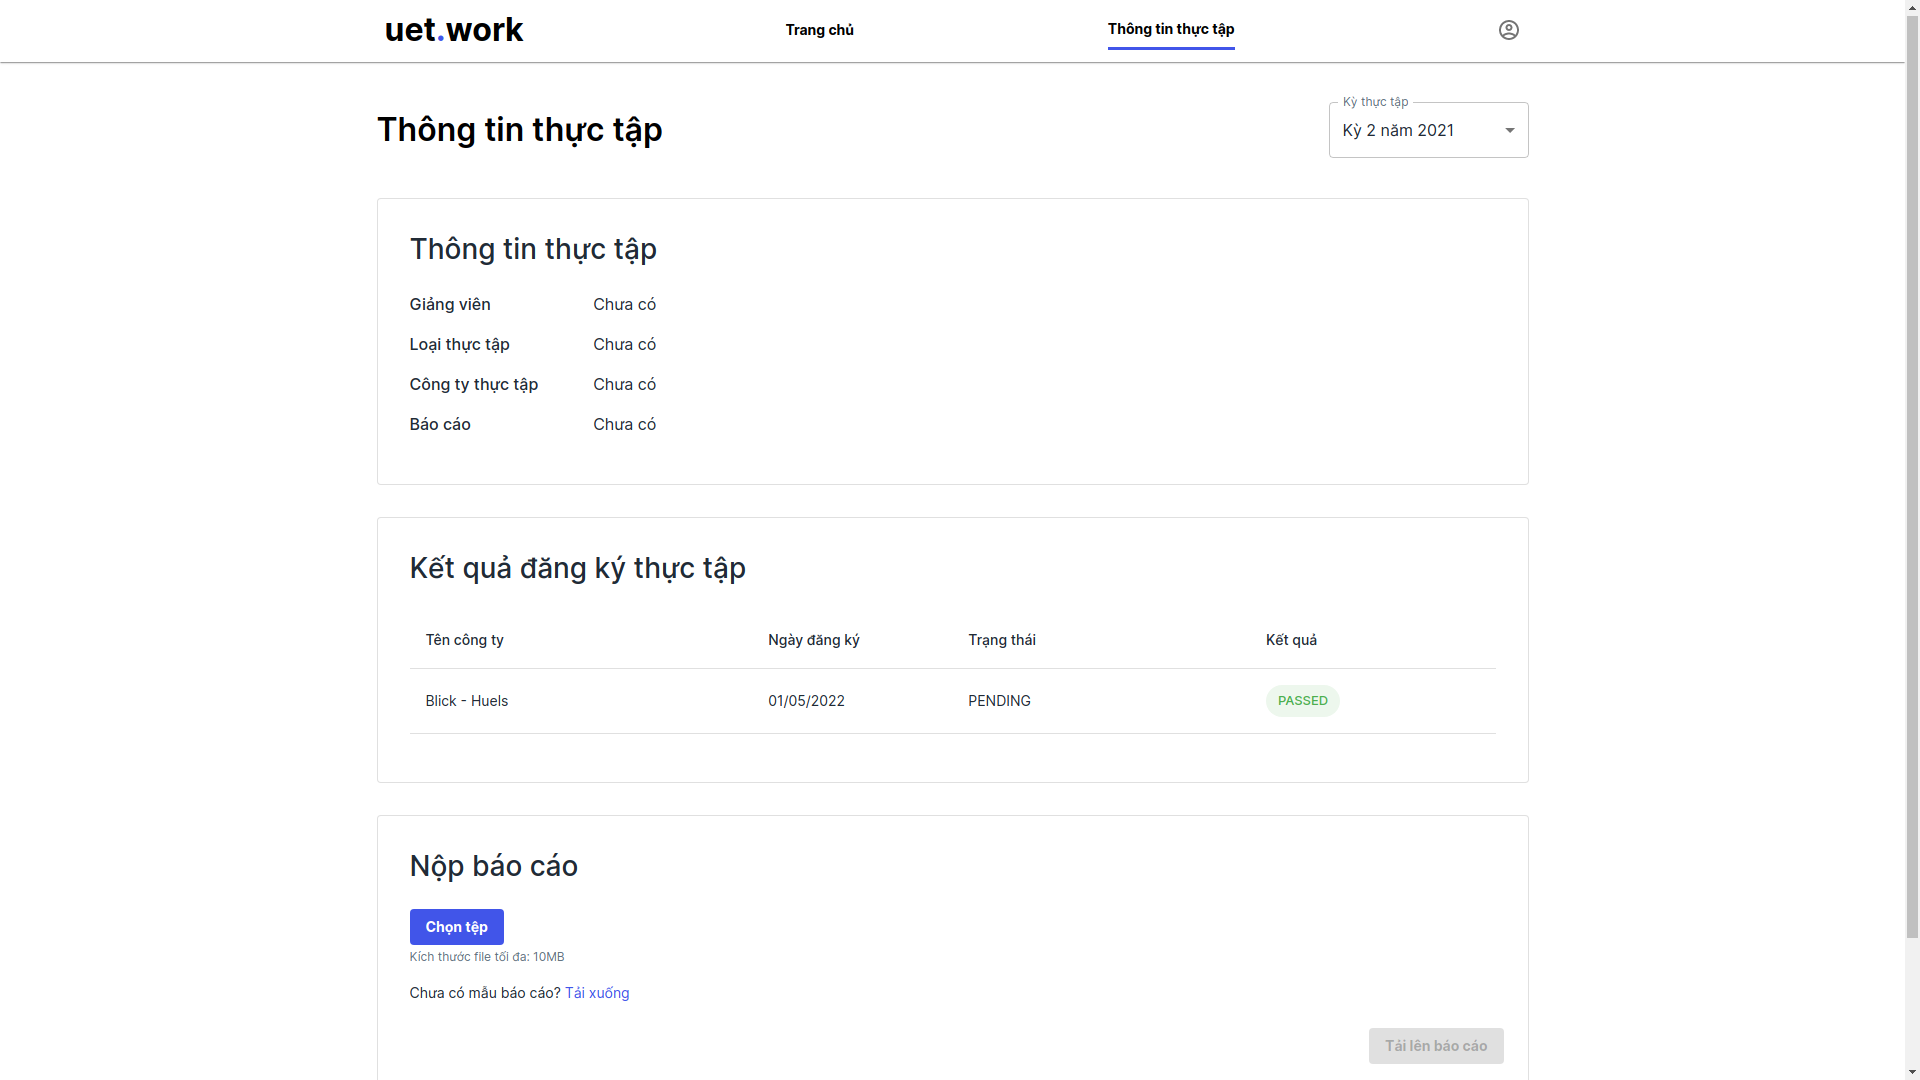
\includegraphics[width=\linewidth]{./images/image17.png}
	\caption{Luồng \emph{Sinh viên xem thông tin thực tập}}
	\label{fig:view_internship_page}
\end{figure}

\subsubsection{Luồng sử dụng của giảng viên}

\paragraph*{Giảng viên xem danh sách sinh viên đang hướng dẫn}

Giảng viên truy cập trang Sinh viên đang hướng dẫn. Tại đây, giảng viên có thể tìm kiếm, sắp xếp, lọc danh sách theo kỳ thực tập, trạng thái báo cáo, trạng thái chấm điểm.

Hình \ref{fig:working_student_page} mô tả màn hình danh sách sinh viên đang hướng dẫn.

\begin{figure}[]
	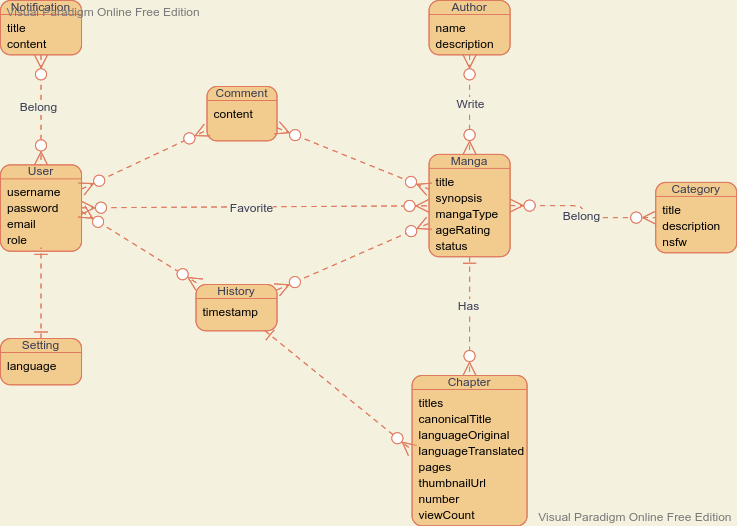
\includegraphics[width=\linewidth]{./images/image8.png}
	\caption{Luồng \emph{Giảng viên xem danh sách sinh viên đang hướng dẫn}}
	\label{fig:working_student_page}
\end{figure}

\paragraph*{Giảng viên tải xuống báo cáo}
Hình \ref{fig:lecturer_access_students}: Giảng viên truy cập trang sinh viên đang hướng dẫn và tải xuống báo cáo của sinh viên.

\begin{figure}[]
	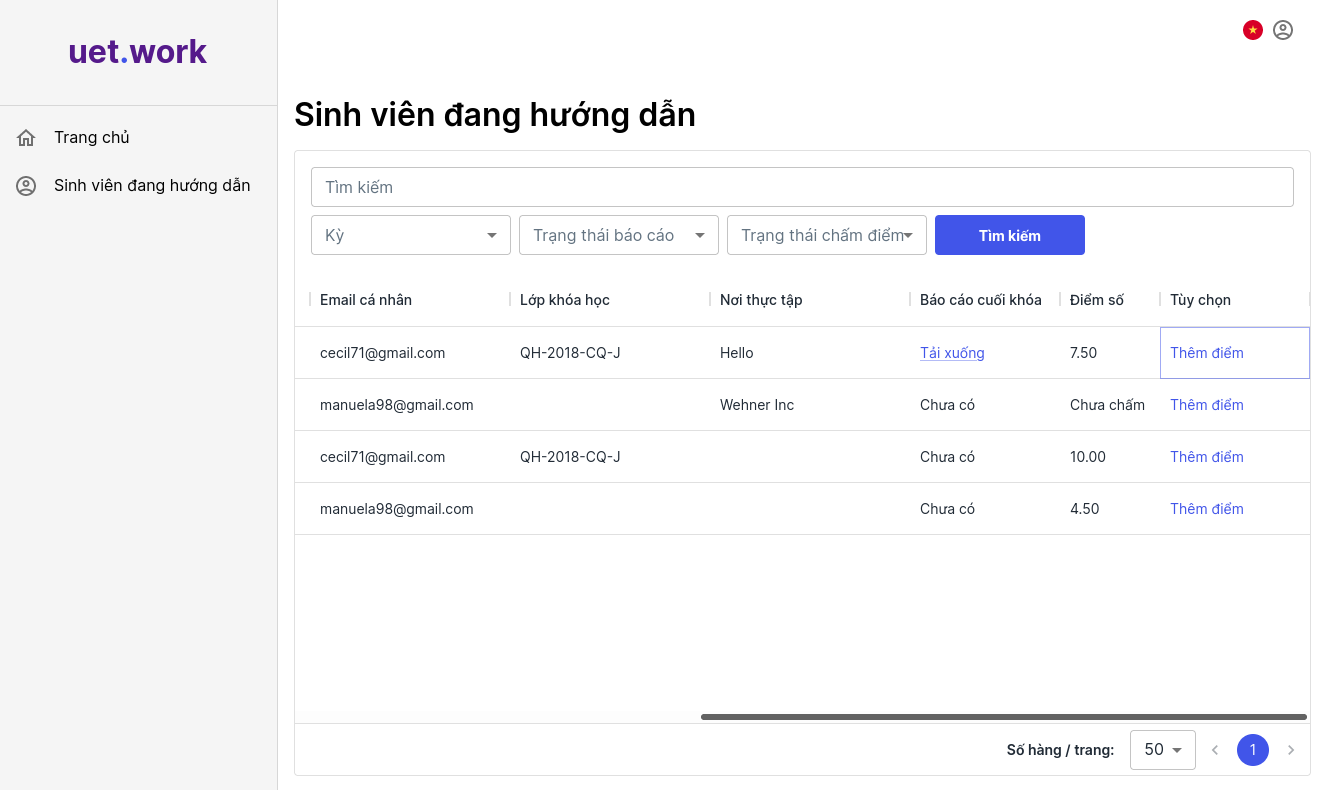
\includegraphics[width=\linewidth]{./images/image64.png}
	\caption{Luồng \emph{Giảng viên tải xuống báo cáo}}
	\label{fig:lecturer_access_students}
\end{figure}

\subsubsection{Luồng sử dụng của đối tác}

\paragraph*{Đối tác xem danh sách bài đăng}

Đối tác truy cập trang Danh sách bài đăng. Tại đây, đối tác có thể tìm kiếm, sắp xếp và lọc danh sách theo kỳ thực tập.

Hình \ref{fig:partner_list_post_page} mô tả màn hình Danh sách bài đăng của đối tác.

\begin{figure}[]
	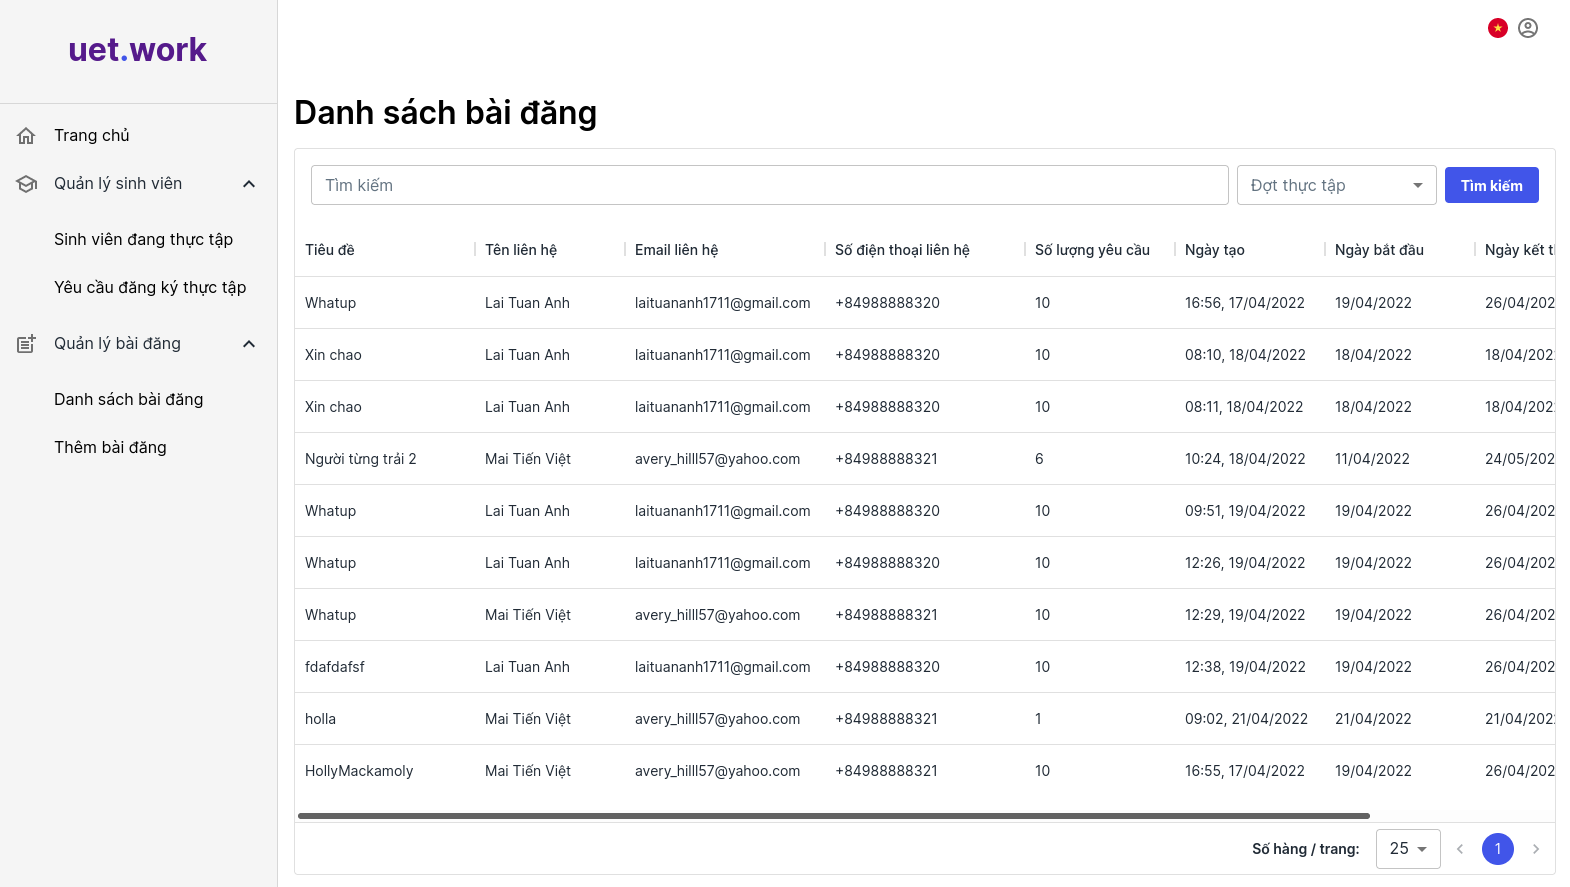
\includegraphics[width=\linewidth]{./images/list_post.png}
	\caption{Luồng \emph{Đối tác xem danh sách bài đăng}}
	\label{fig:partner_list_post_page}
\end{figure}

\paragraph*{Đối tác thêm bài đăng tuyển dụng}

Tại trang Thêm bài đăng, đối tác thêm tiêu đề, nội dung chi tiết, số lượng tuyển dụng, ngày bắt đầu, ngày kết thúc, người liên hệ để tạo một bài đăng mới.

Hình \ref{fig:add_post_page} mô tả màn hình thêm bài đăng của đối tác.

\begin{figure}[]
	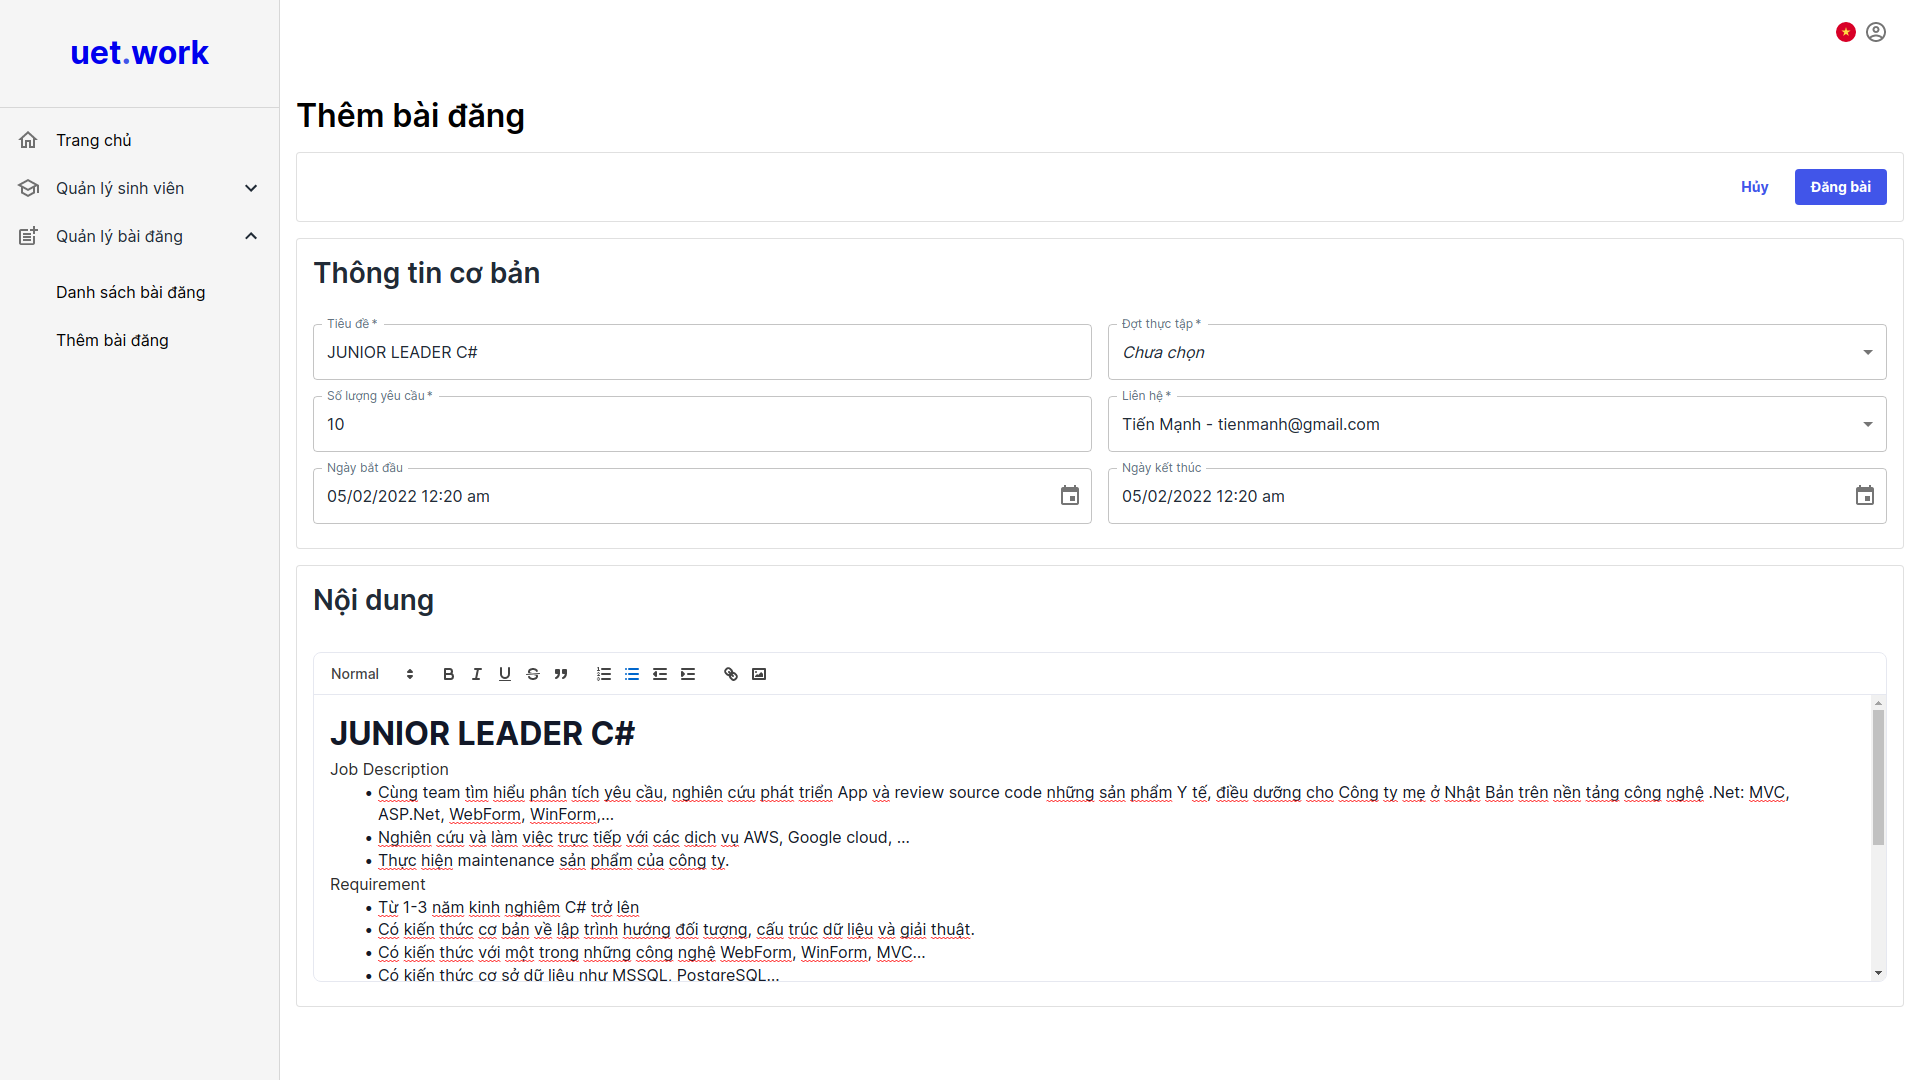
\includegraphics[width=\linewidth]{./images/image18.png}
	\caption{Luồng \emph{Đối tác thêm bài đăng tuyển dụng}}
	\label{fig:add_post_page}
\end{figure}

\paragraph*{Đối tác xem danh sách yêu cầu đăng ký thực tập}

Đối tác truy cập trang Yêu cầu đăng ký thực tập. Tại đây, đối tác có thể tìm kiếm, sắp xếp, lọc danh sách theo kỳ thực tập và chấp nhận / từ chối sinh viên.

Hình \ref{fig:partner_view_list_requests_page} mô tả màn hình danh sách yêu cầu đăng ký thực tập.

\begin{figure}[]
	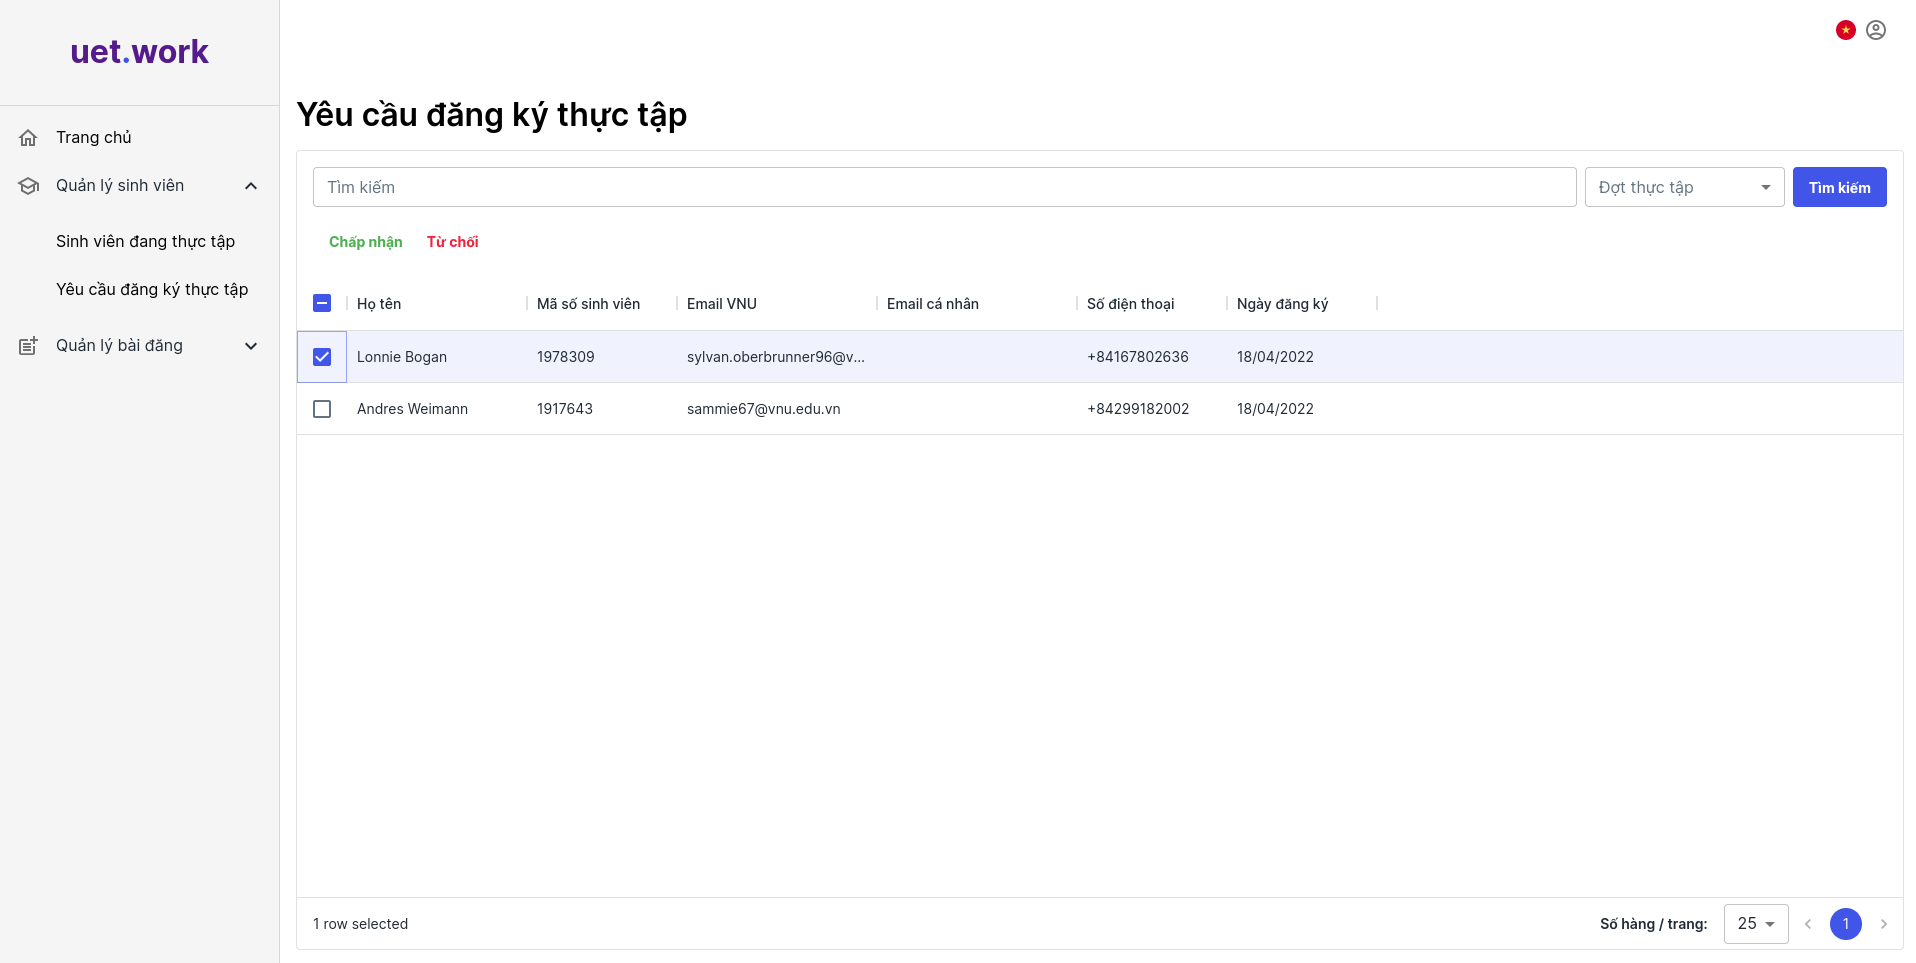
\includegraphics[width=\linewidth]{./images/image29.png}
	\caption{Luồng \emph{Đối tác xem danh sách yêu cầu đăng ký thực tập}}
	\label{fig:partner_view_list_requests_page}
\end{figure}

\subsubsection{Luồng sử dụng của quản trị viên Khoa}

\paragraph*{Quản trị viên Khoa tạo kỳ thực tập mới}

\begin{itemize}
	\item Hình \ref{fig:org_admin_access_list_terms}: Quản trị viên Khoa truy cập trang Danh sách kỳ thực tập.
	\item Hình \ref{fig:org_admin_add_term}: Quản trị viên Khoa thực hiện tạo kỳ thực tập mới.
	\item Hình \ref{fig:org_admin_add_term_success}: Tạo kỳ thực tập thành công.
\end{itemize}

\begin{figure}[]
	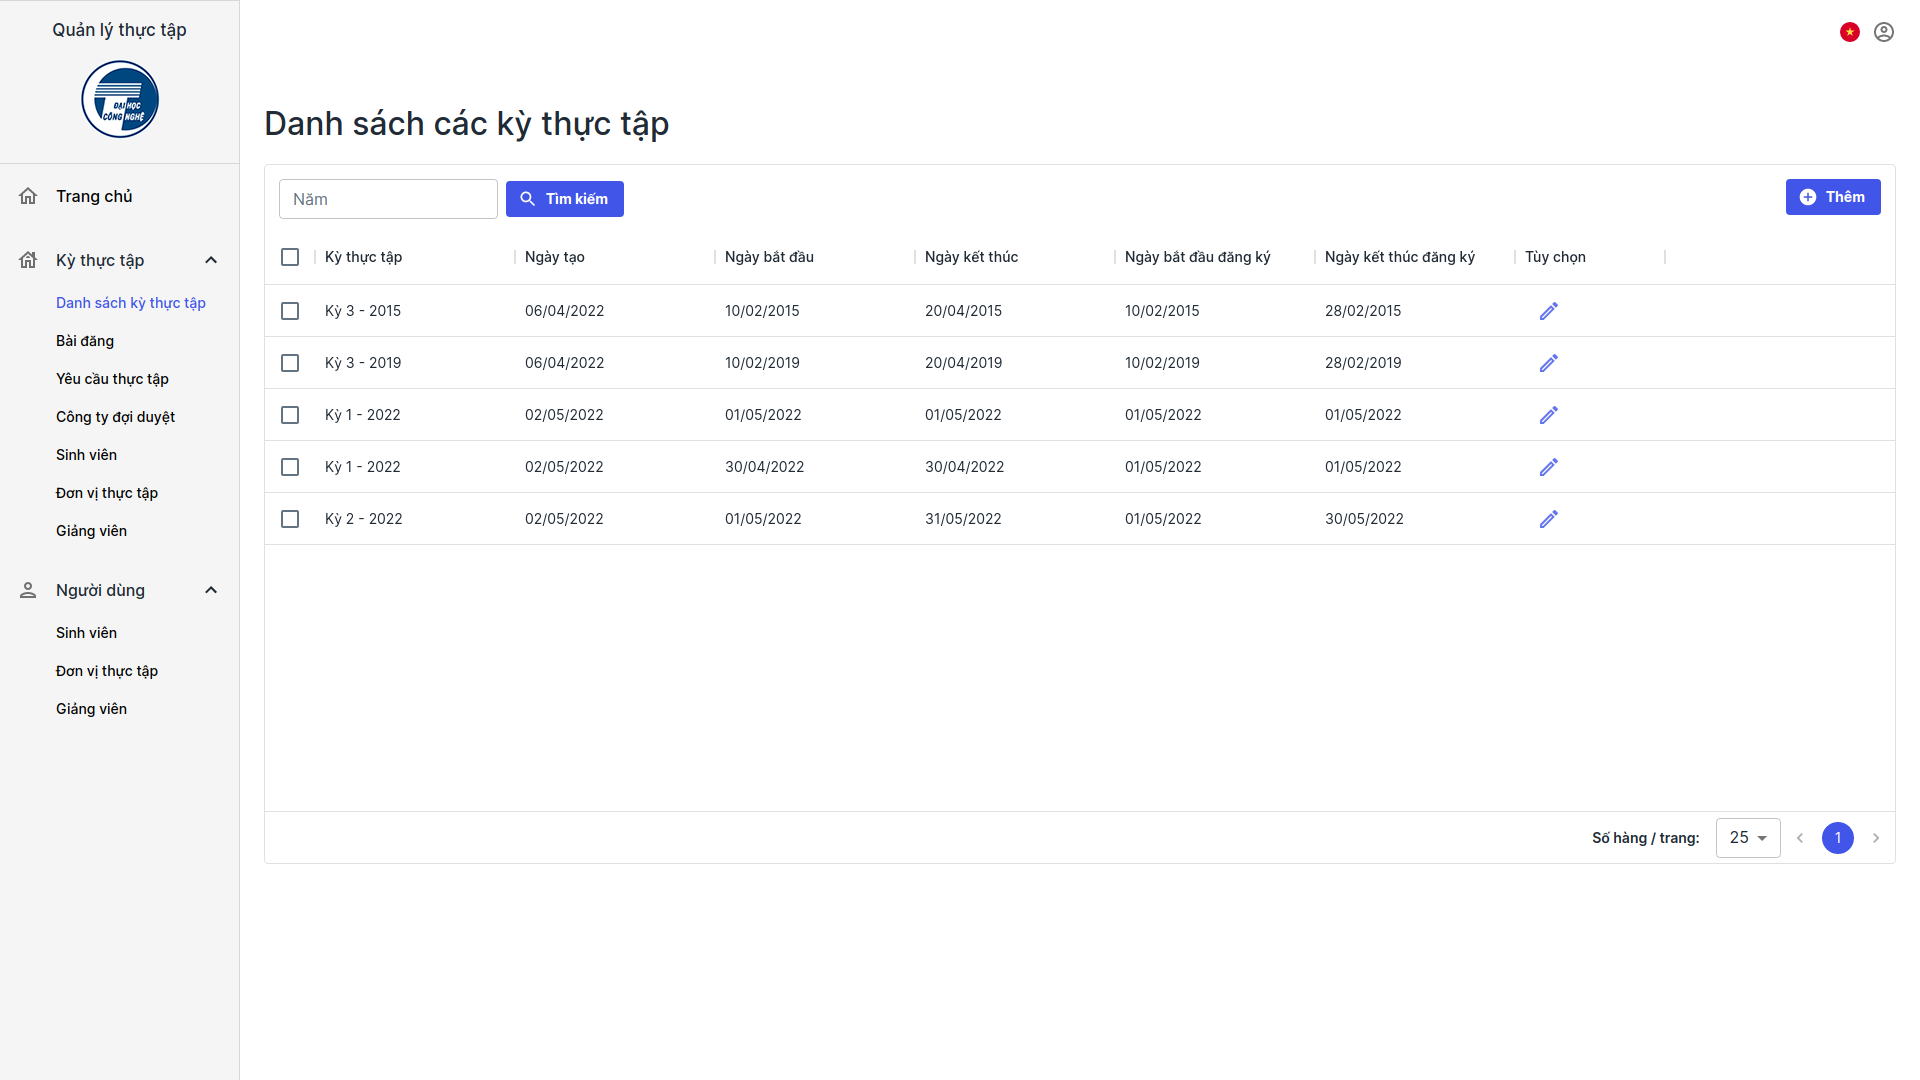
\includegraphics[width=\linewidth]{./images/image53.png}
	\caption{Luồng \emph{Quản trị viên Khoa tạo kỳ thực tập mới}: Truy cập trang Danh sách kỳ thực tập}
	\label{fig:org_admin_access_list_terms}
\end{figure}

\begin{figure}[]
	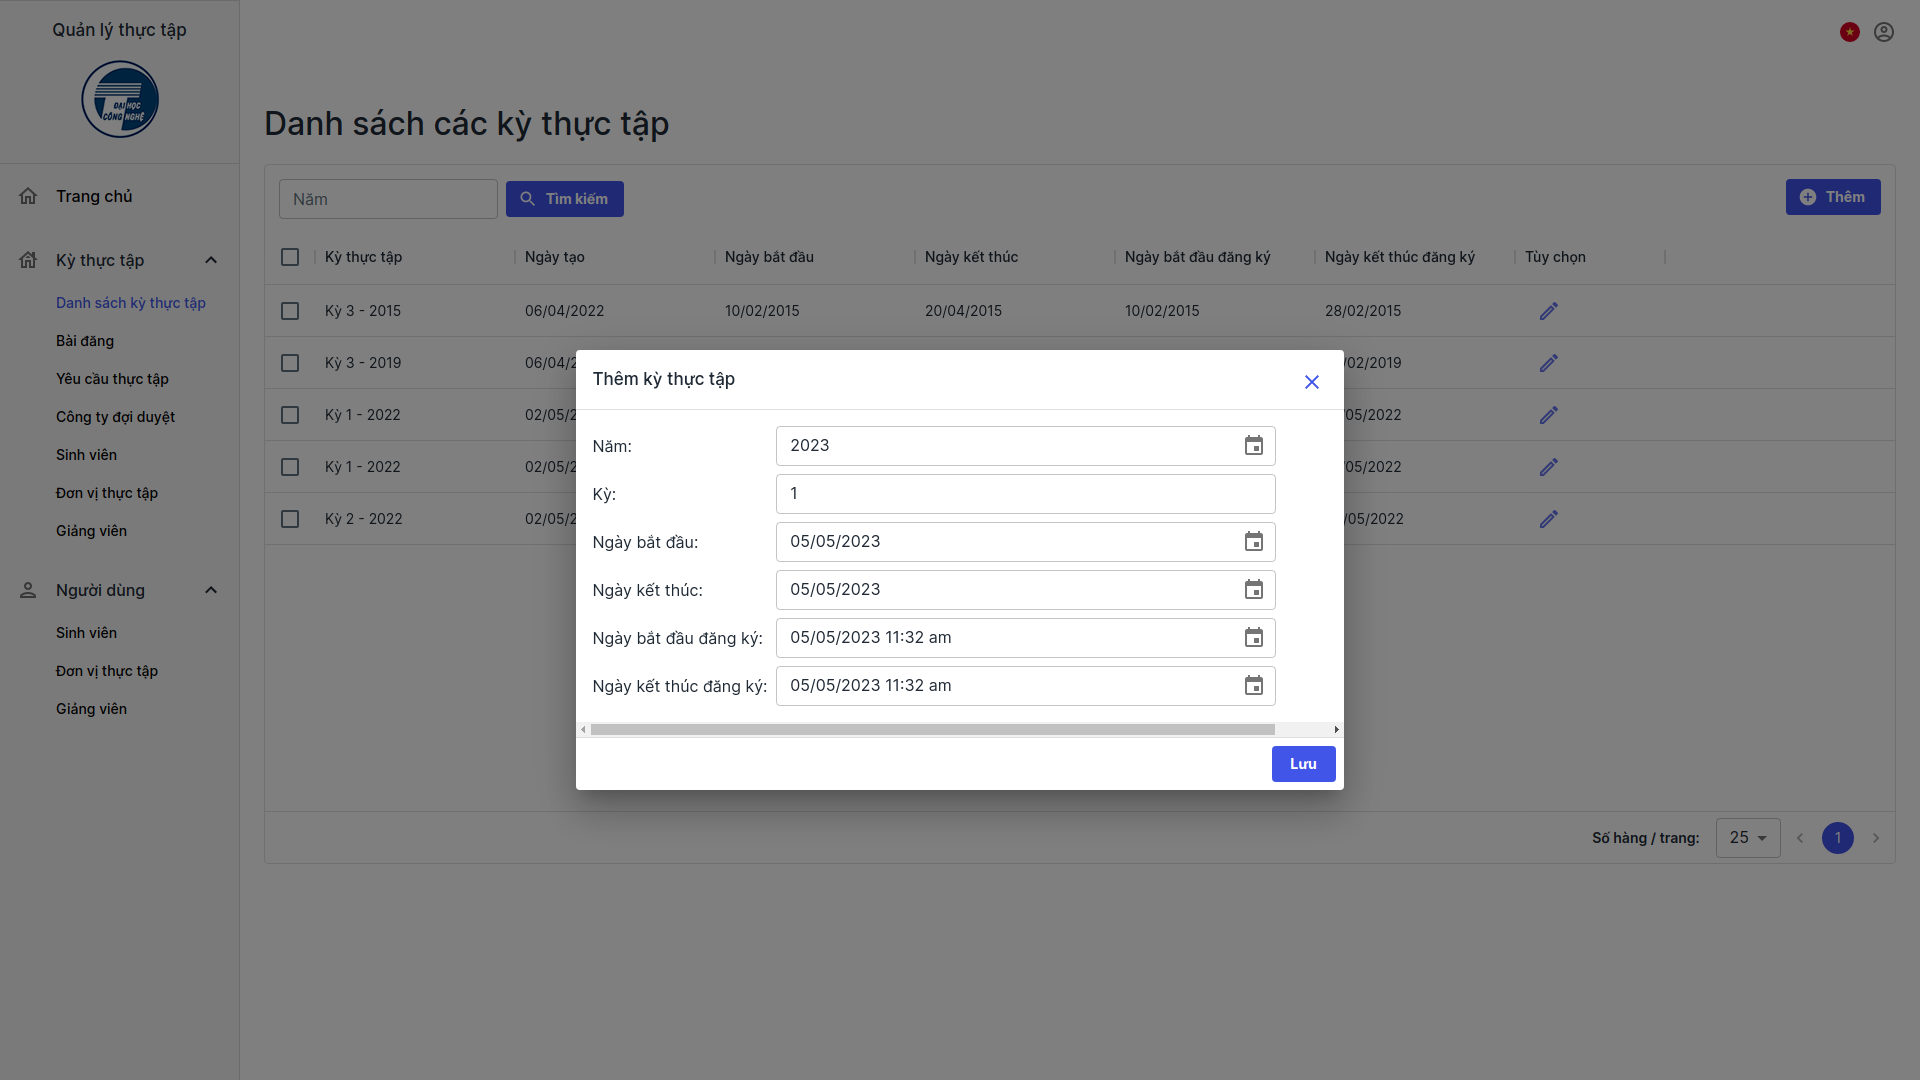
\includegraphics[width=\linewidth]{./images/image54.png}
	\caption{Luồng \emph{Quản trị viên Khoa tạo kỳ thực tập mới}: Thực hiện tạo kỳ thực tập mới}
	\label{fig:org_admin_add_term}
\end{figure}

\begin{figure}[]
	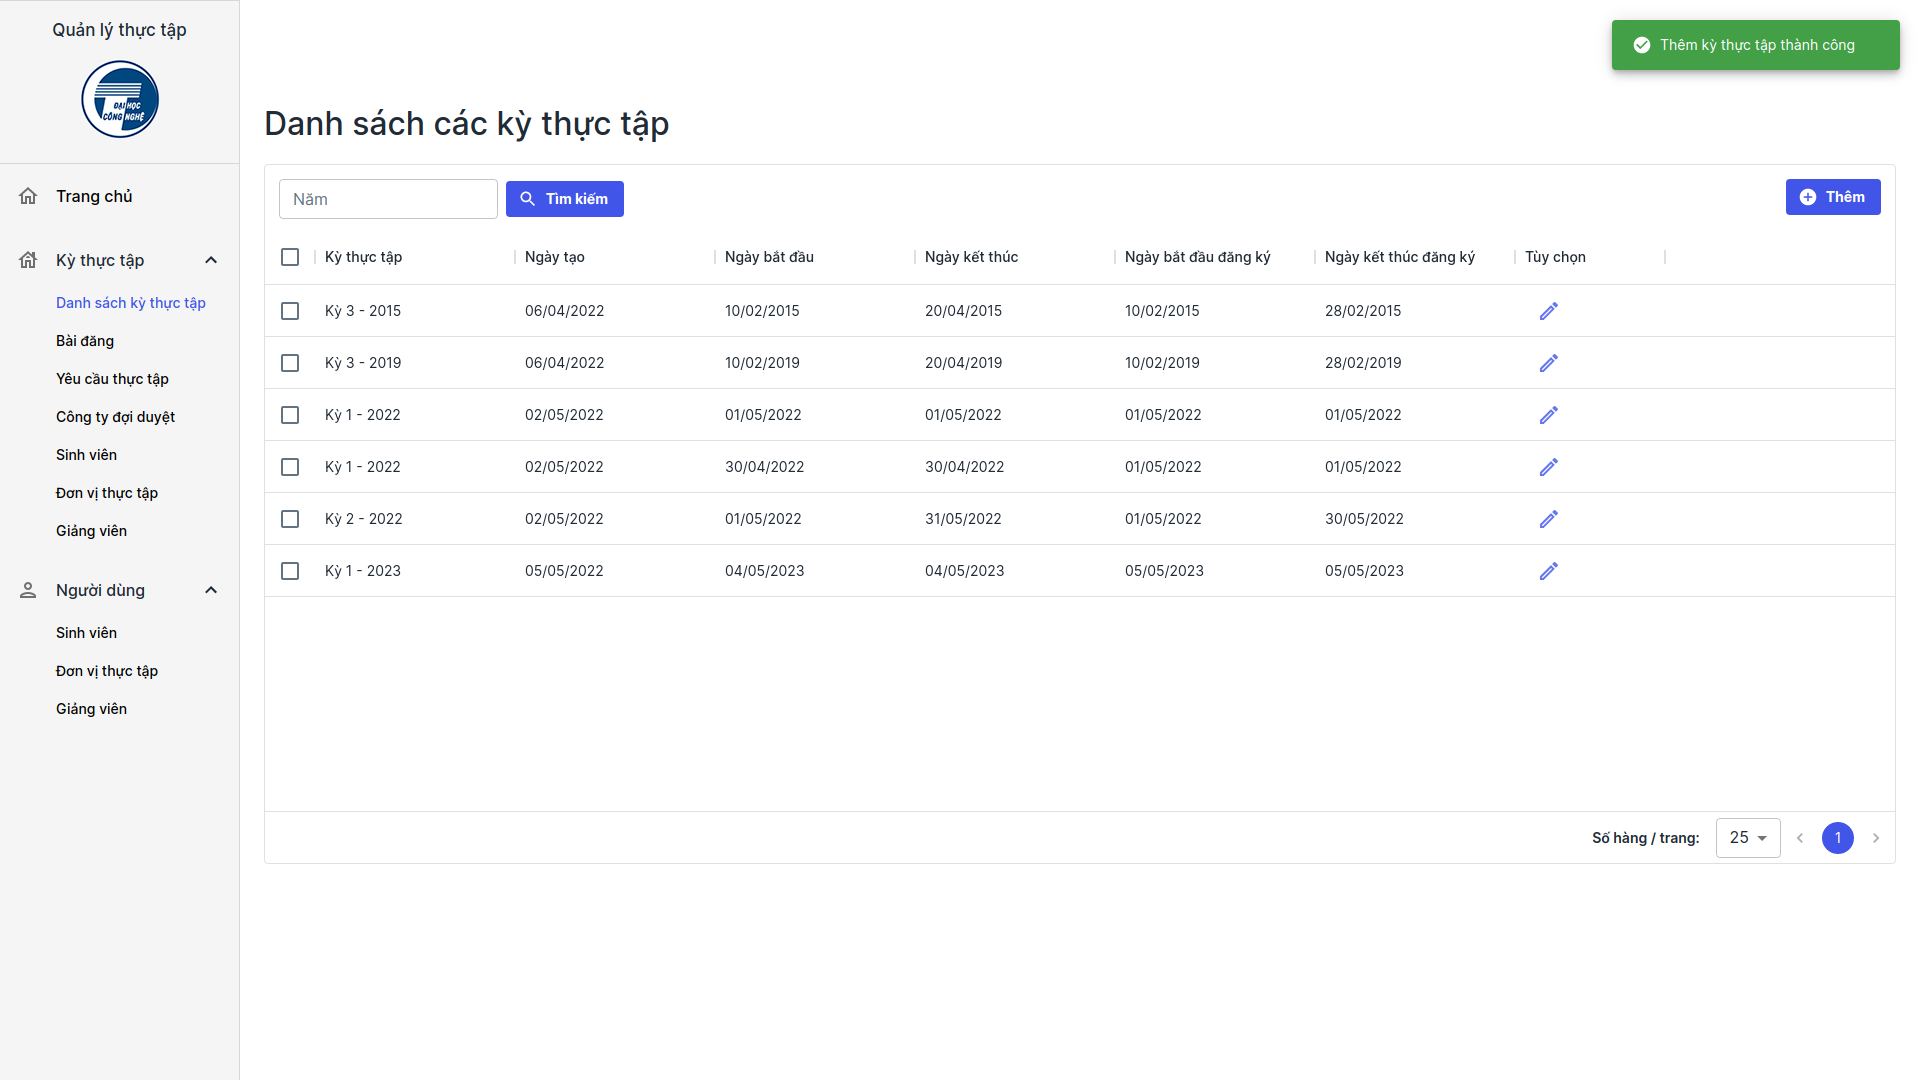
\includegraphics[width=\linewidth]{./images/image55.png}
	\caption{Luồng \emph{Quản trị viên Khoa tạo kỳ thực tập mới}: Tạo kỳ thực tập thành công}
	\label{fig:org_admin_add_term_success}
\end{figure}

\paragraph*{Quản trị viên Khoa xem danh sách bài đăng của các đối tác}

Quản trị viên truy cập trang danh sách Bài đăng. Tại đây, quản trị viên có thể tìm kiếm, sắp xếp danh sách, thêm, sửa bài đăng cho đối tác.

Hình \ref{fig:orgadmin_list_posts} mô tả màn hình danh sách bài đăng của các đối tác.

\begin{figure}[]
	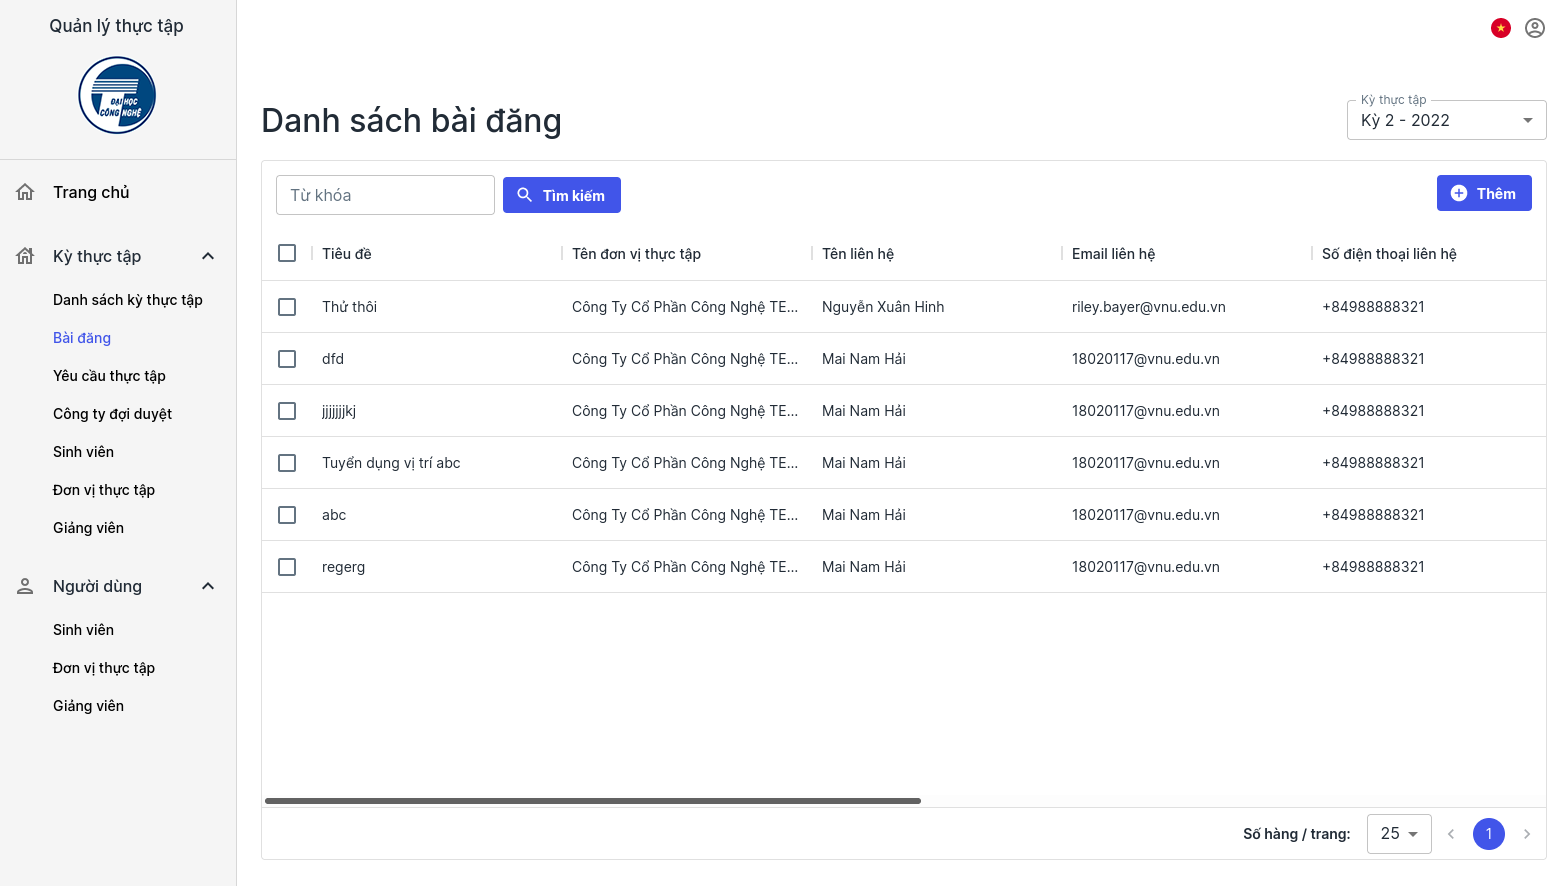
\includegraphics[width=\linewidth]{./images/image71.png}
	\caption{Luồng \emph{Quản trị viên Khoa xem danh sách bài đăng của các đối tác}}
	\label{fig:orgadmin_list_posts}
\end{figure}

\paragraph*{Quản trị viên Khoa chấp nhận / từ chối yêu cầu thực tập}

\begin{itemize}
	\item Hình \ref{fig:org_admin_access_list_requests}: Quản trị viên truy cập trang Yêu cầu thực tập trong kỳ thực tập.
	\item Hình \ref{fig:org_admin_select_requests}: Quản trị viên chọn danh sách sinh viên và chọn tùy chọn Chấp nhận / Từ chối.
\end{itemize}

\begin{figure}[]
	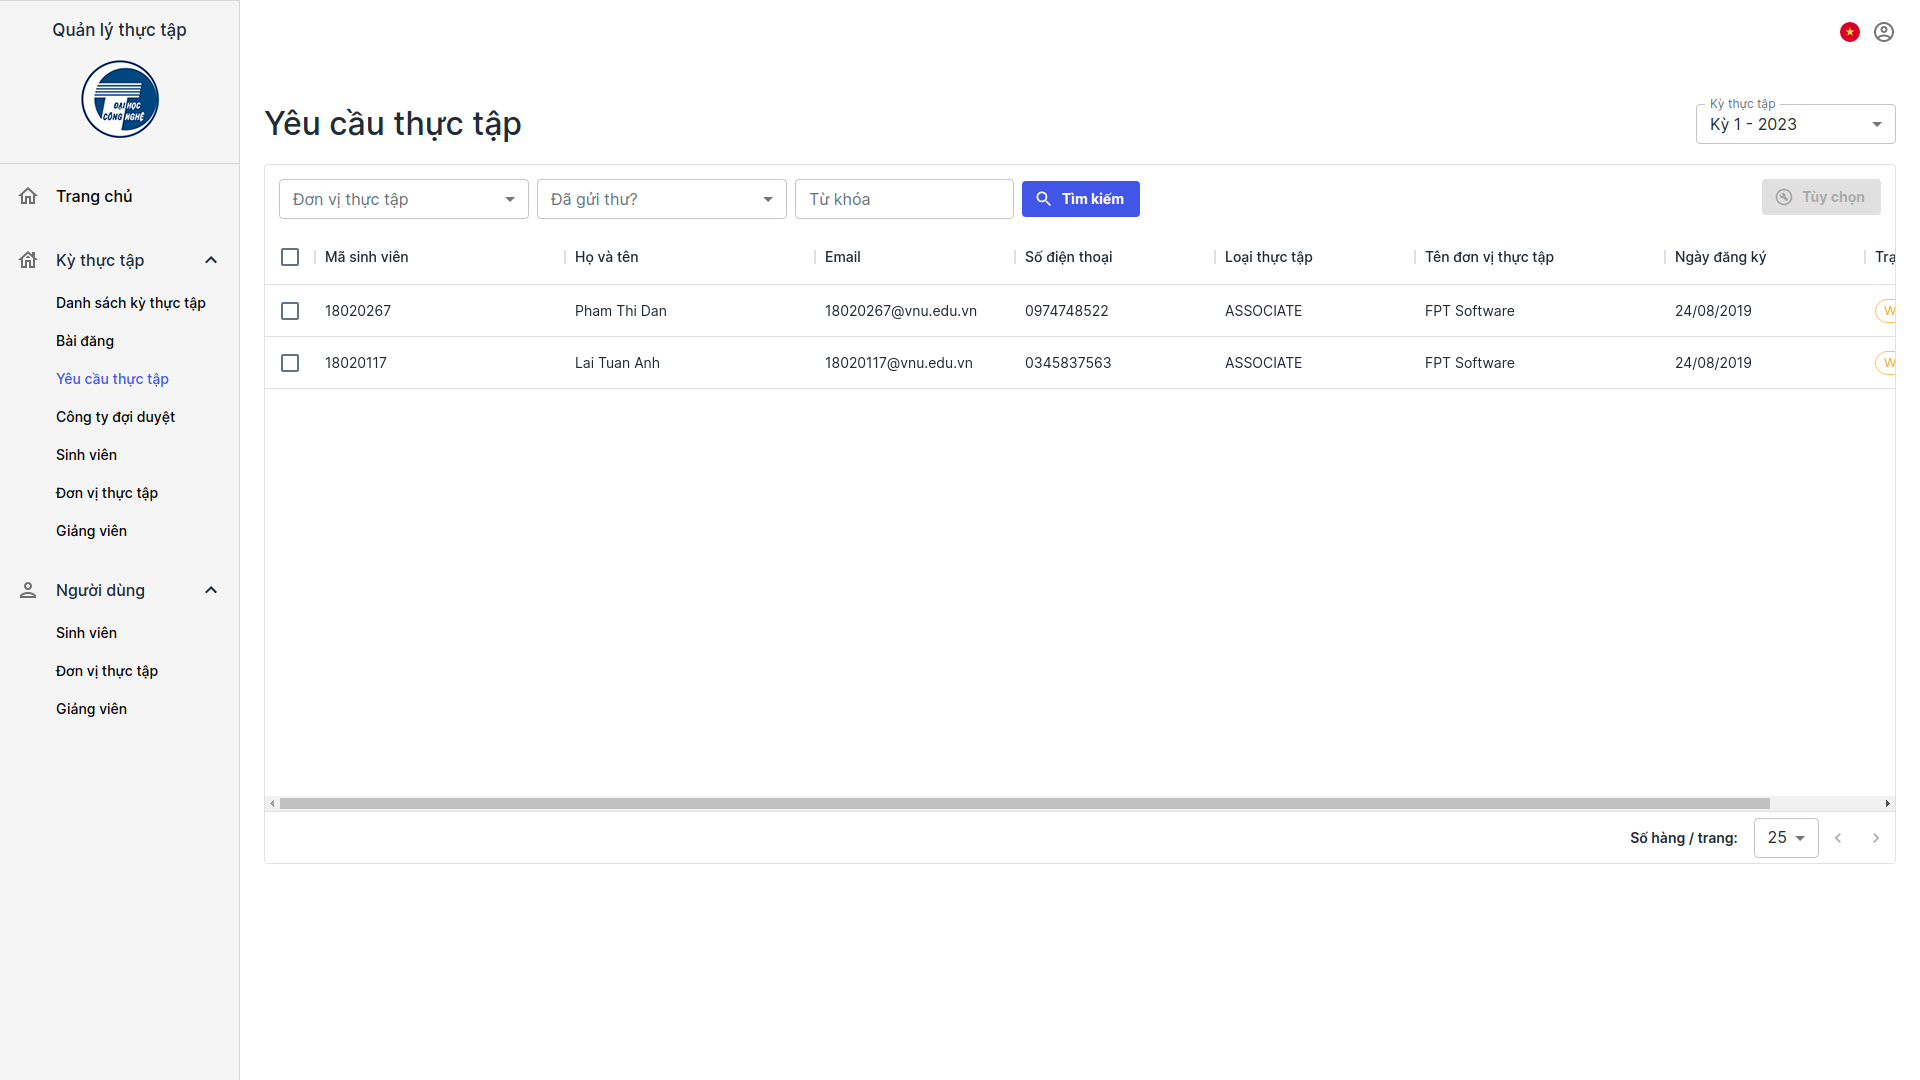
\includegraphics[width=\linewidth]{./images/image72.png}
	\caption{Luồng \emph{Quản trị viên Khoa Chấp nhận / từ chối yêu cầu thực tập}: truy cập danh sách yêu cầu thực tập}
	\label{fig:org_admin_access_list_requests}
\end{figure}

\begin{figure}[]
	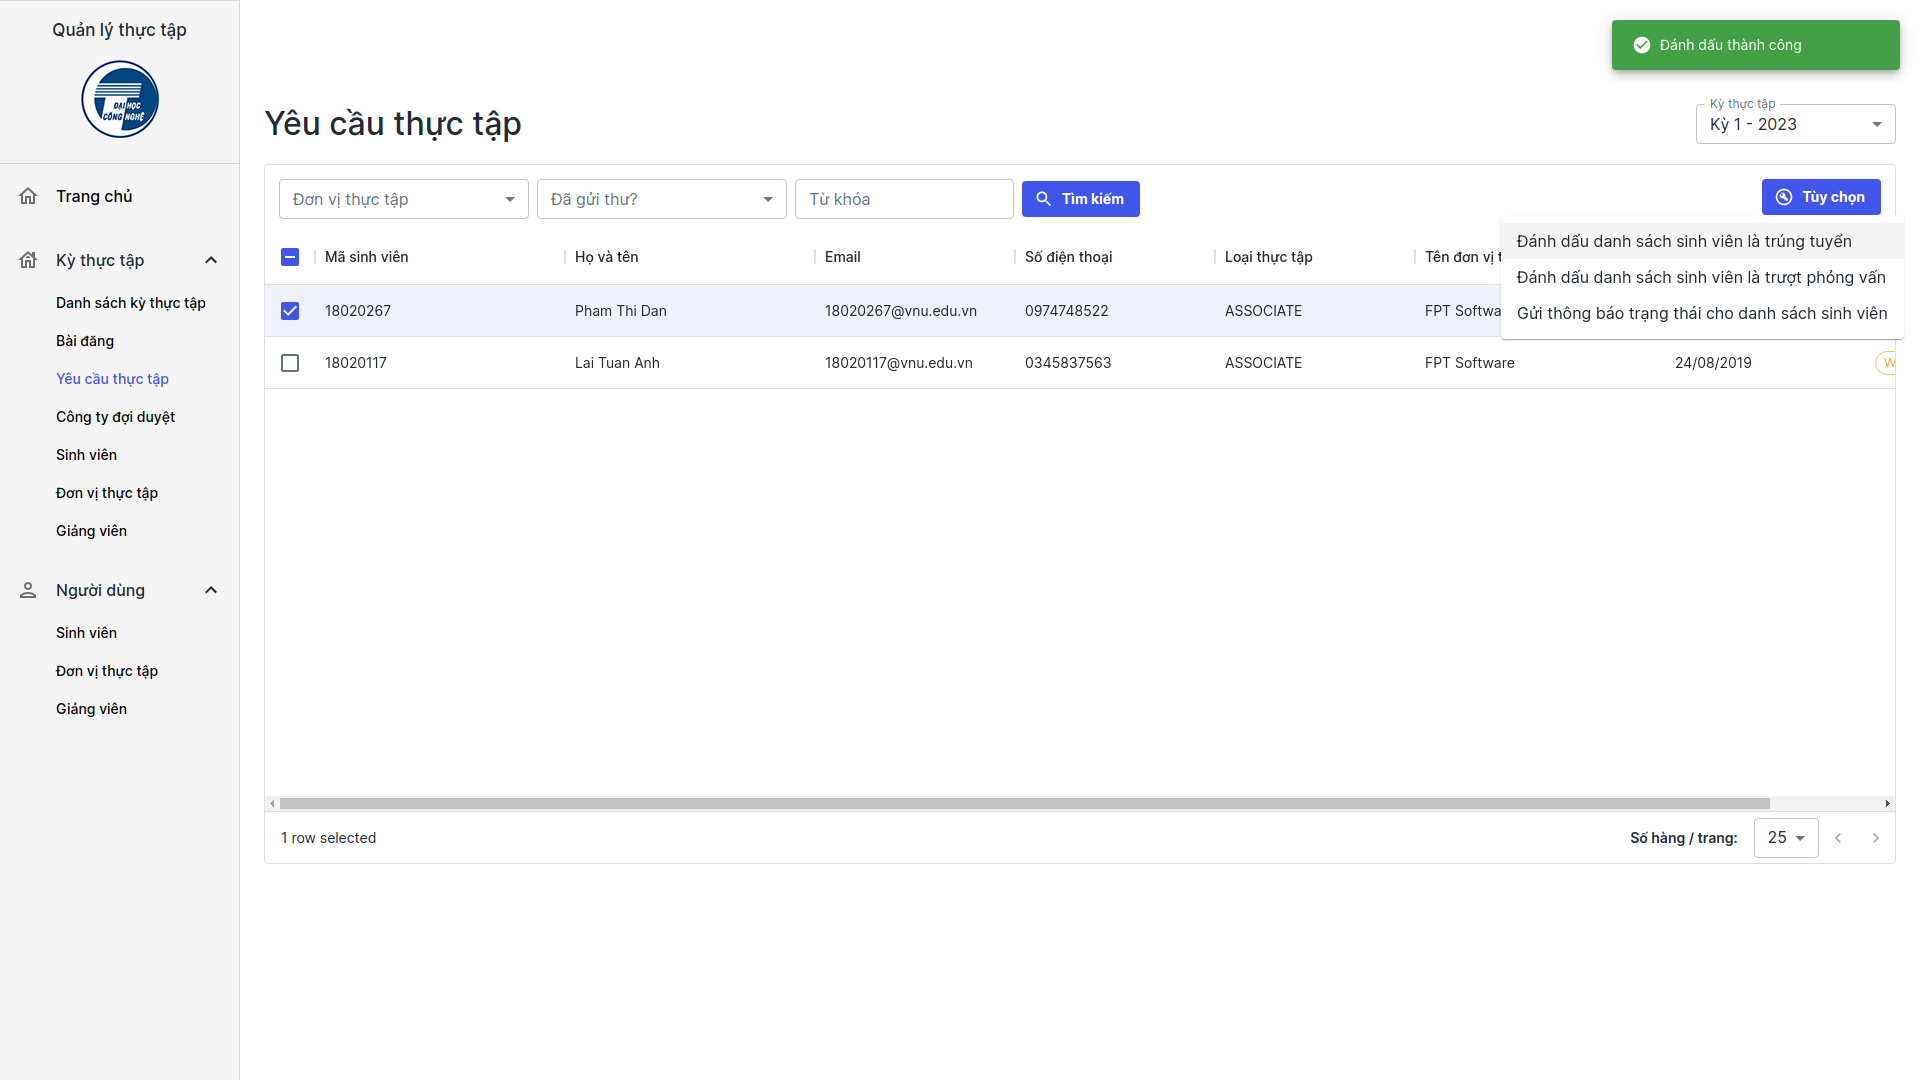
\includegraphics[width=\linewidth]{./images/image73.png}
	\caption{Luồng \emph{Quản trị viên Khoa chấp nhận / từ chối yêu cầu thực tập}: chọn danh sách sinh viên và chọn Chấp nhận / Từ chối}
	\label{fig:org_admin_select_requests}
\end{figure}

\subsubsection{Luồng sử dụng của quản trị viên hệ thống}

\paragraph*{Quản trị viên tạo Khoa mới}

\begin{itemize}
	\item Hình \ref{fig:admin_access_list_orgs}: Quản trị viên truy cập danh sách Khoa.
	\item Hình \ref{fig:admin_add_org}: Quản trị viên chọn Thêm Khoa mới và thực hiện tạo mới.
	\item Hình \ref{fig:admin_add_org_success}: Tạo mới thành công.
\end{itemize}

\begin{figure}[]
	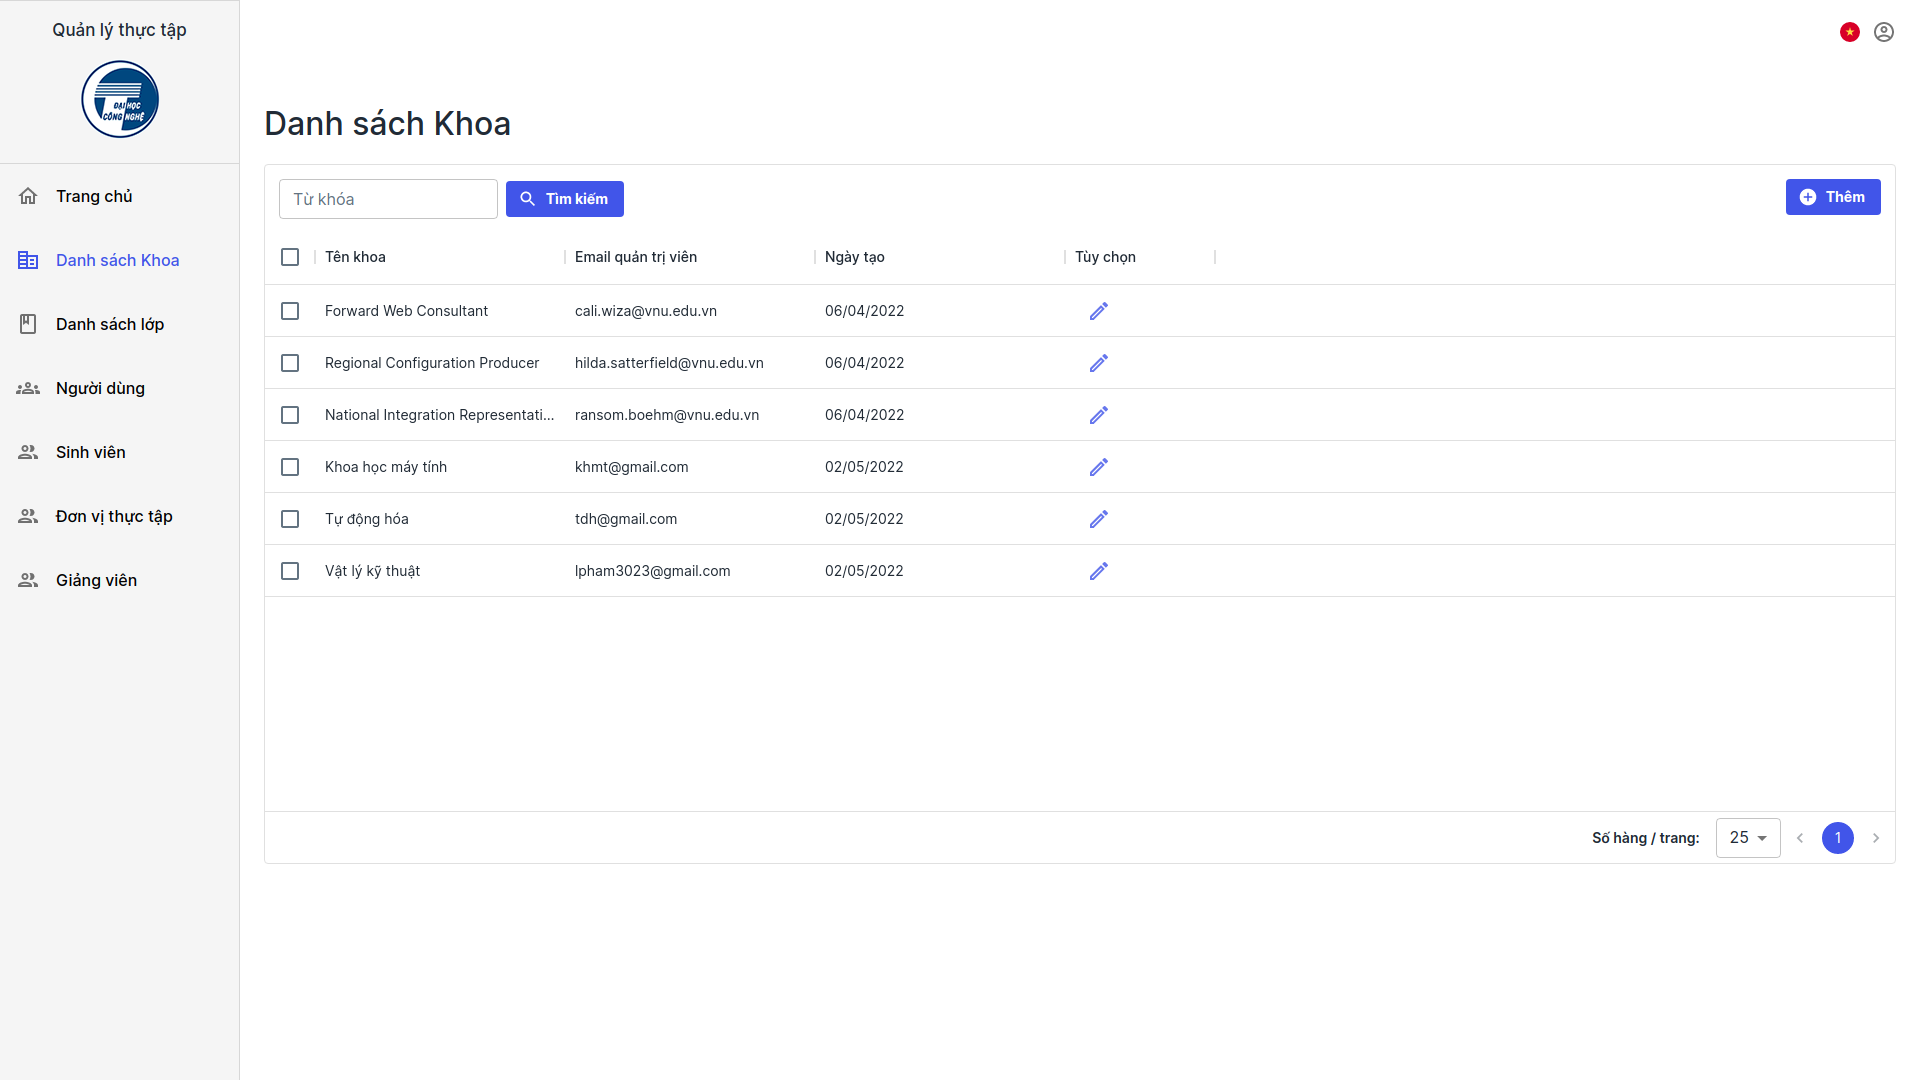
\includegraphics[width=\linewidth]{./images/image56.png}
	\caption{Luồng \emph{Quản trị viên tạo Khoa mới}: truy cập danh sách Khoa}
	\label{fig:admin_access_list_orgs}
\end{figure}

\begin{figure}[]
	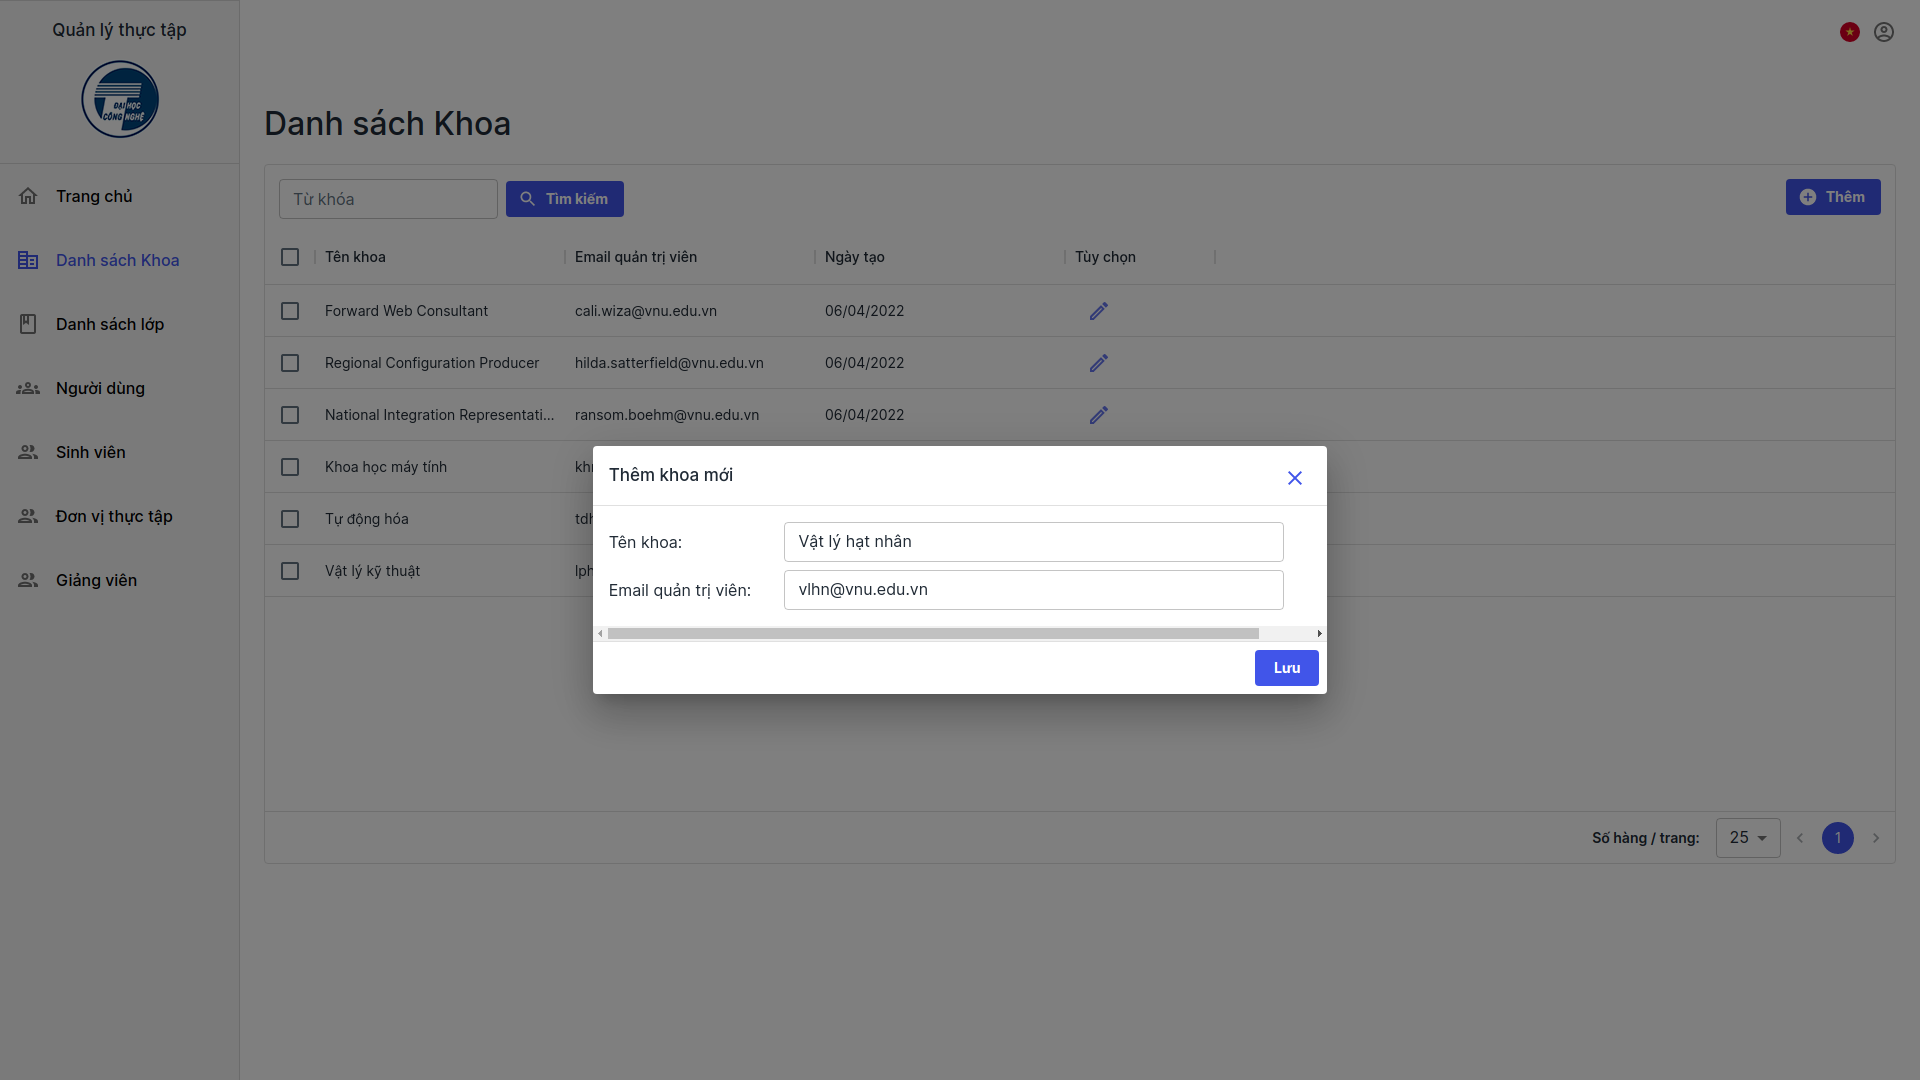
\includegraphics[width=\linewidth]{./images/image57.png}
	\caption{Luồng \emph{Quản trị viên tạo Khoa mới}: chọn Thêm Khoa mới và thực hiện tạo mới}
	\label{fig:admin_add_org}
\end{figure}

\begin{figure}[]
	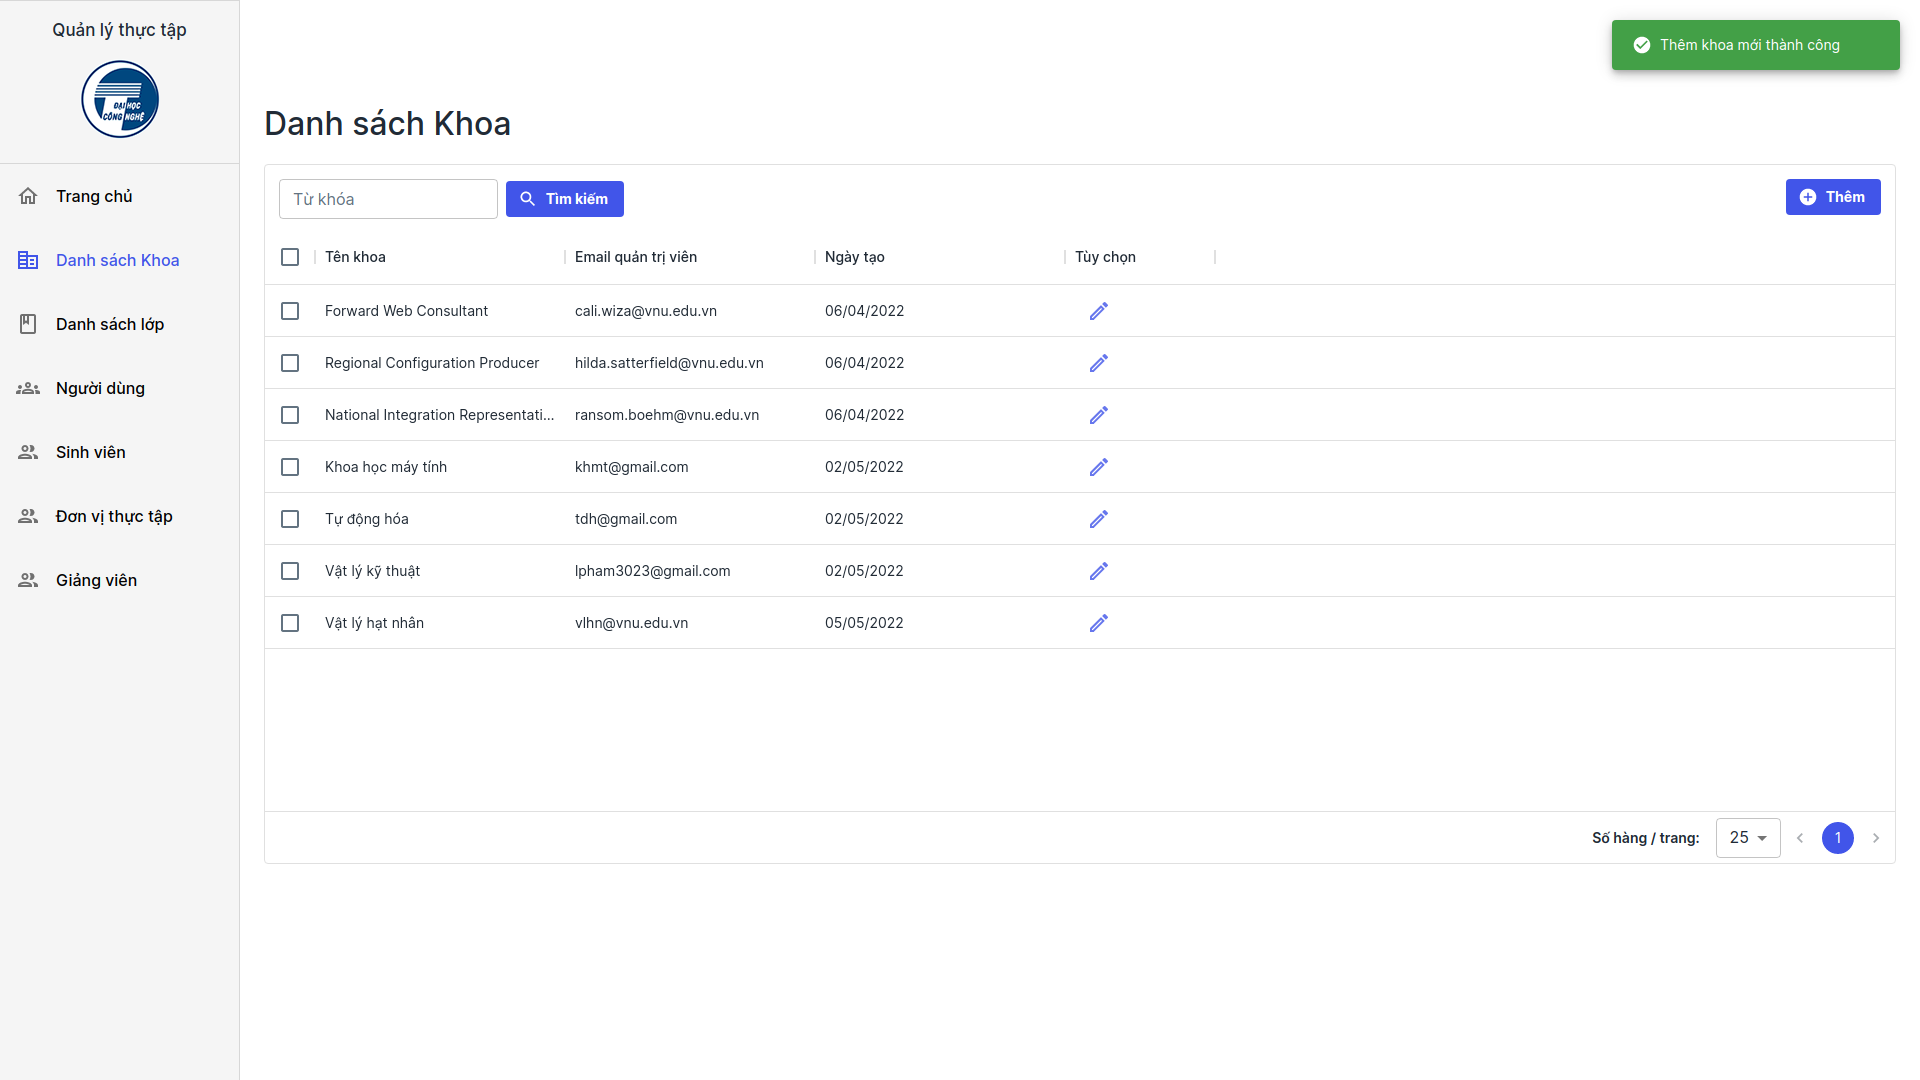
\includegraphics[width=\linewidth]{./images/image58.png}
	\caption{Luồng \emph{Quản trị viên tạo Khoa mới}: Tạo mới thành công}
	\label{fig:admin_add_org_success}
\end{figure}

\paragraph*{Quản trị viên tạo Lớp mới}

\begin{itemize}
	\item Hình \ref{fig:admin_access_list_classes}: Quản trị viên truy cập danh sách lớp.
	\item Hình \ref{fig:admin_add_class}: Quản trị viên chọn Thêm lớp và thực hiện tạo mới.
	\item Hình \ref{fig:admin_add_class_success}: Tạo mới thành công.
\end{itemize}

\begin{figure}[]
	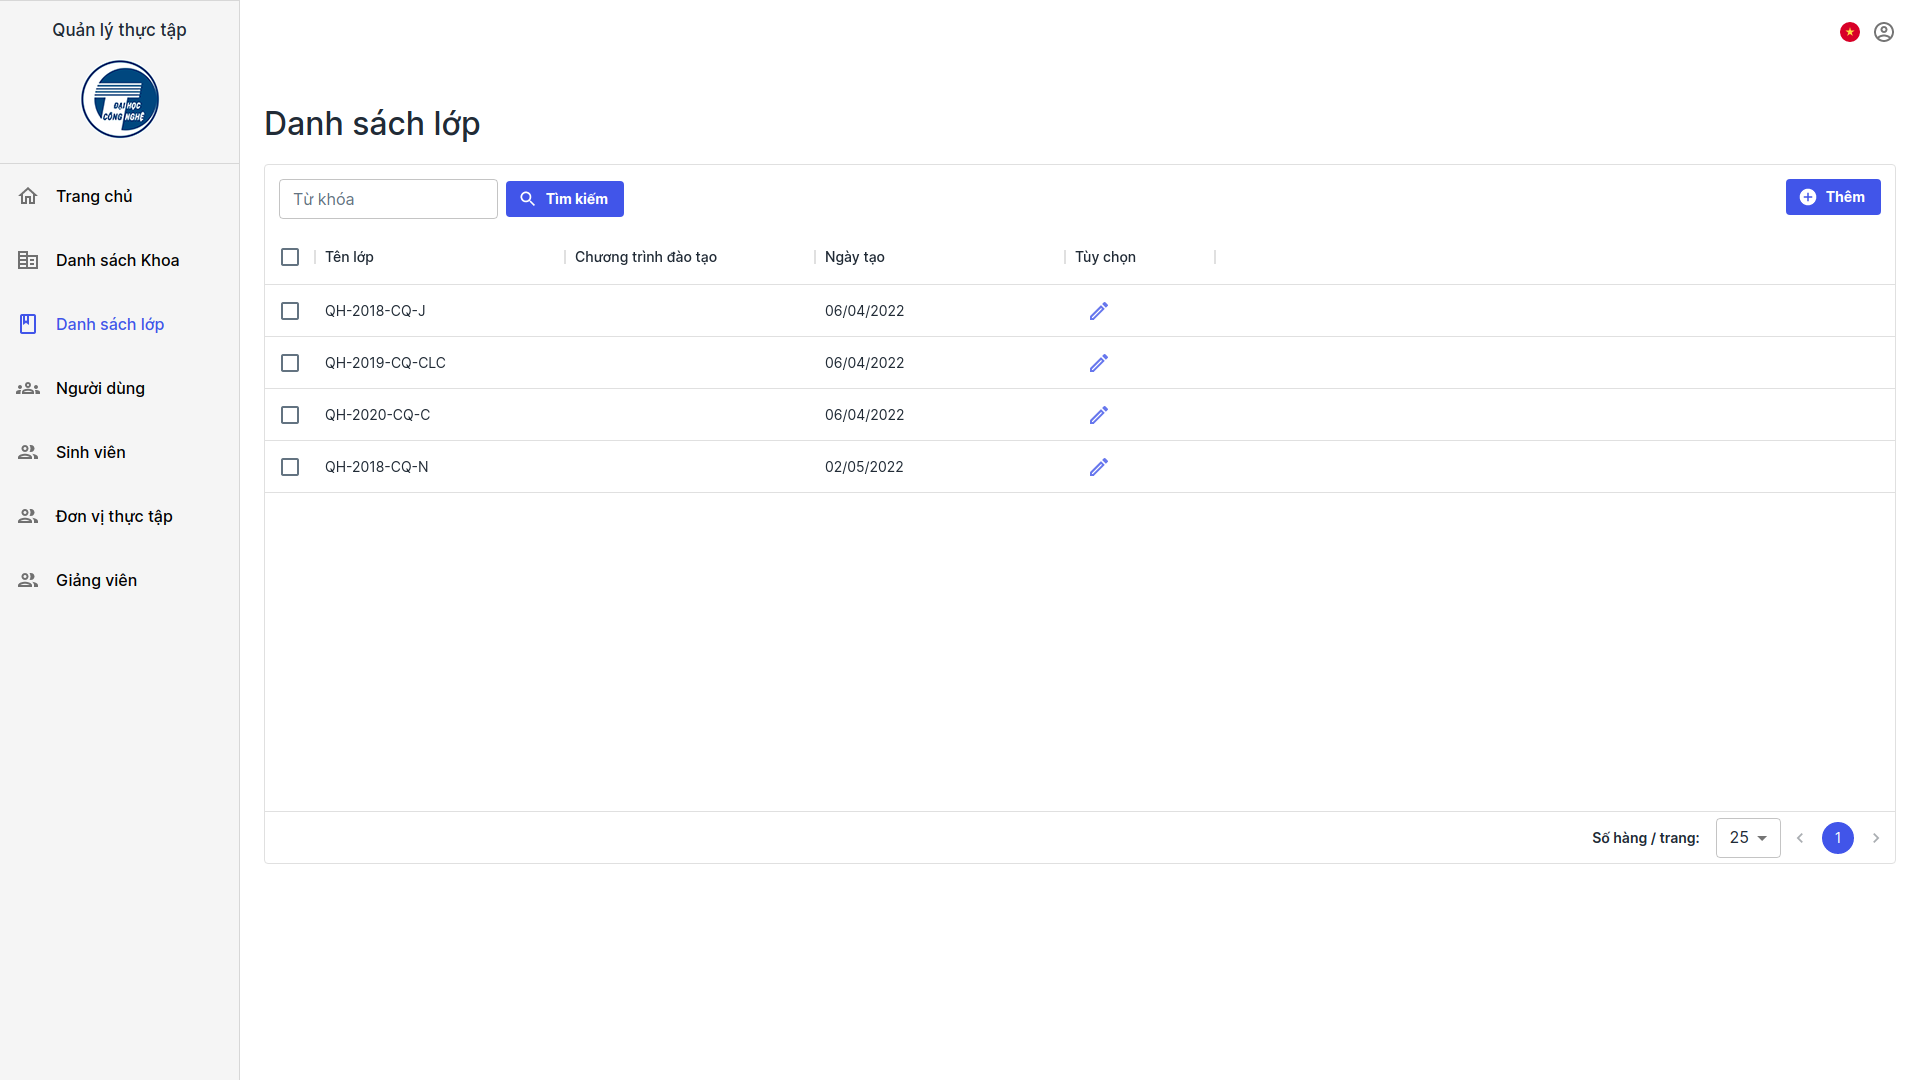
\includegraphics[width=\linewidth]{./images/image59.png}
	\caption{Luồng \emph{Quản trị viên tạo Lớp mới}: truy cập danh sách Lớp}
	\label{fig:admin_access_list_classes}
\end{figure}

\begin{figure}[]
	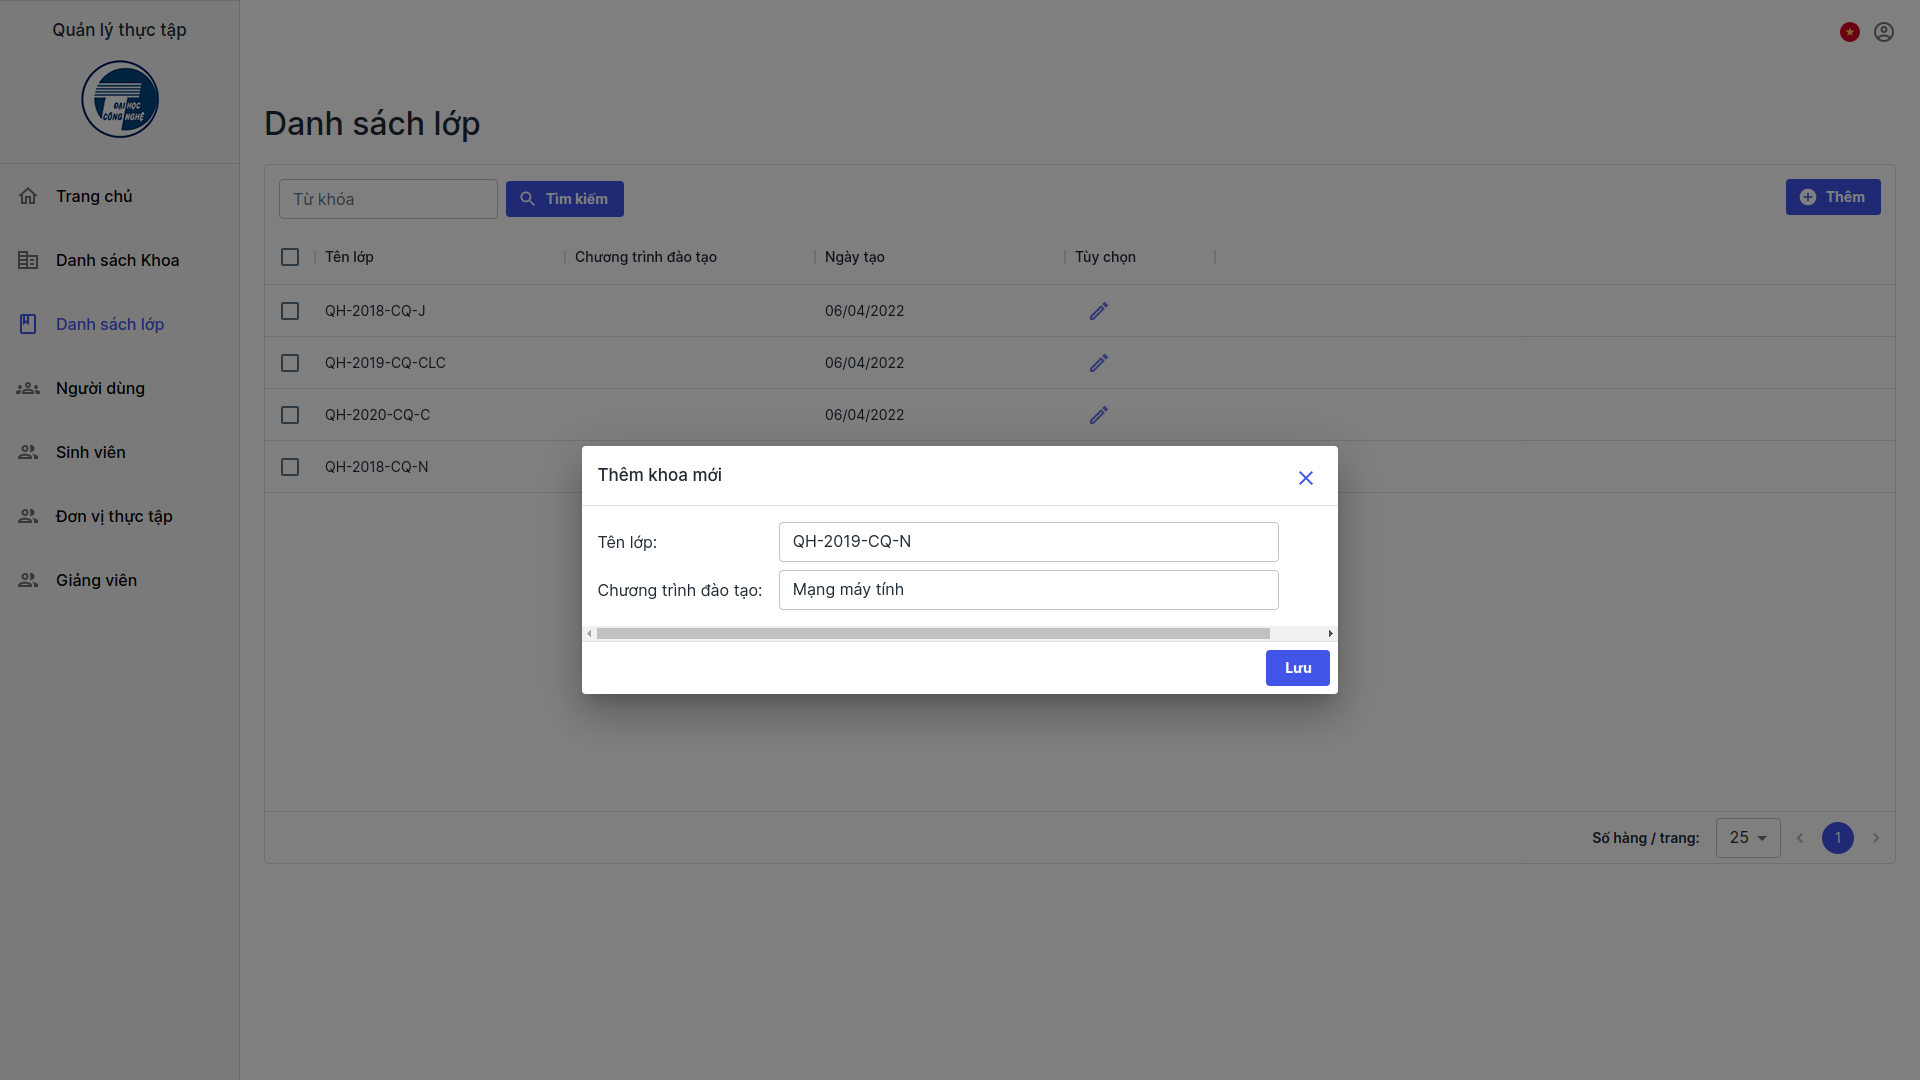
\includegraphics[width=\linewidth]{./images/image60.png}
	\caption{Luồng \emph{Quản trị viên tạo Lớp mới}: chọn Thêm Lớp mới và thực hiện tạo mới}
	\label{fig:admin_add_class}
\end{figure}

\begin{figure}[]
	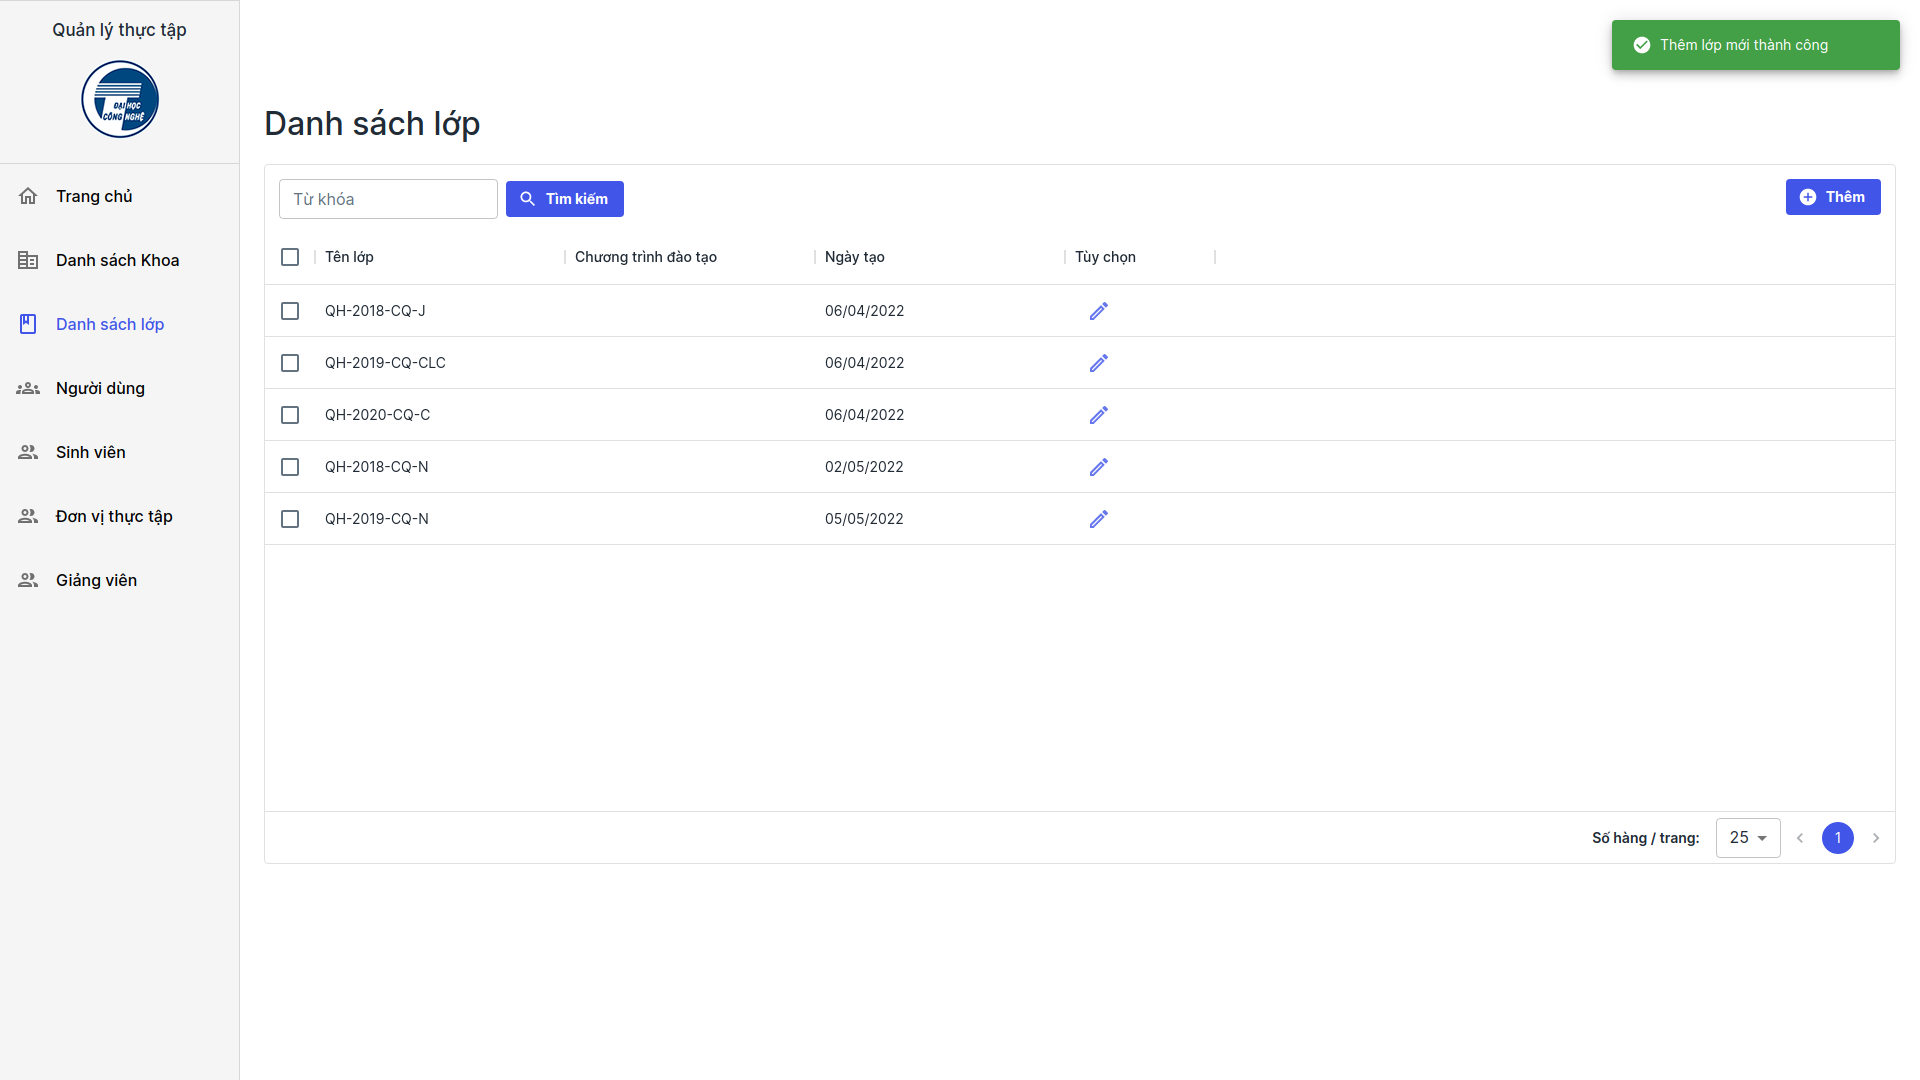
\includegraphics[width=\linewidth]{./images/image61.png}
	\caption{Luồng \emph{Quản trị viên tạo Lớp mới}: Tạo mới thành công}
	\label{fig:admin_add_class_success}
\end{figure}

\end{document}